\documentclass[12pt,a4paper]{report}
\usepackage[margin=25mm]{geometry}
\usepackage[T1]{fontenc}
\usepackage[utf8]{inputenc}
\usepackage{lmodern}
\usepackage{amsmath,amssymb}
\usepackage{flafter}
\usepackage{float}
\usepackage{tikz}
\usetikzlibrary{arrows.meta}
\usepackage[hidelinks]{hyperref}
\begin{document}
\setcounter{chapter}{3}
\chapter{Evidence-Aware Evaluation of Question Decomposition}
\label{ch:evidence-aware}
\label{chap:empirical-studies}

\section*{Introduction}

Once a decision to decompose a question has been made, the challenge is to
turn its subquestions into useful retrieval and reading steps. Evaluating 
that process requires knowing where the annotated evidence appears and estimating 
which subquestions are responsible for retrieving it. Following Chapter~3's study 
of compositional difficulty,this chapter develops an evidence-aware framework for 
evaluating the execution of a decomposition.

The framework combines a matrix of evidence ranks with a learned ownership
model. It measures complete evidence availability, the depth required by
assigned subquestions, and the answers produced during execution. We validate
the ownership predictor on reference-style decompositions and compare direct
retrieval with generated decomposition on $100$ MuSiQue questions. A second
analysis examines how a fixed passage budget can be distributed across the
retrieval lists, including BM25 experiments on three benchmarks.

These studies establish three foundations for Chapter~5. The ownership-masked
score supplies an objective for prompt optimisation. Balanced and oracle
allocations quantify the opportunity for learned passage selection. The
distinction between evidence availability, assignment, and answer execution
provides the structure for diagnostic feedback. The chapter develops these
foundations in turn, from measurement and validation to retrieval results and
budget analysis.

\section{Problem Formulation}
\label{sec:ch4-problem}

\subsection{Sequential Execution of a Decomposition}

Let $q$ be a question with reference answer $y$ and annotated supporting
passages $E(q)=\{e_1,\ldots,e_h\}$. MuSiQue supplies both supporting passages
and a reference decomposition into connected single-hop questions
\cite{trivedi2022musique}. A generated decomposition is an ordered sequence
$U(q)=(u_1,\ldots,u_A)$. An item $u_a$ may contain a reference to the answer of
an earlier item. The execution substitutes the predicted earlier answer,
retrieves passages for the resulting query $\widetilde u_a$ and produces an
intermediate answer $\widehat y_a$:
\begin{equation}
  \widetilde u_a
  = \operatorname{substitute}(u_a,\widehat y_1,\ldots,\widehat y_{a-1}),
  \qquad
  \widehat y_a
  = \operatorname{reader}\bigl(\widetilde u_a,R_a[1:k]\bigr).
  \label{eq:ch4-execution}
\end{equation}
Here $R_a=(d_{a1},d_{a2},\ldots)$ is the ranked passage list returned for
$\widetilde u_a$, and $k$ is the number of passages supplied to the reader.
Backward references make the execution sequential even when the decomposition
contains conceptually independent branches. The retained implementation returns
$\widehat y_A$ as the final answer. Each step receives its own retrieved
context; the final step has no additional synthesis call over the union of all
earlier passages. One such step, a resolved query with its retrieval and its
reader call, is an arm of the execution.

The number of generated subquestions $A$ may differ from the reference hop
count $h$. One subquestion can combine several reference information needs.
Several subquestions can address the same need. The evaluation therefore permits
many-to-many assignments instead of requiring an alignment by position.

\subsection{Evaluation Requirements}

A useful decomposition must make the supporting evidence available, direct it
to the subquestions that need it, and produce the requested answer. We
distinguish these requirements as follows.
\begin{description}
  \item[Availability.] Every annotated supporting passage occurs in at least
  one retrieved prefix.
  \item[Assignment.] Every supporting passage has an identified owner, and
  each owning subquestion retrieves the passages assigned to it.
  \item[Execution.] The reader produces the required intermediate answers
  and the final answer matches the reference under the specified answer metric.
\end{description}

These properties answer different questions. Evidence retrieved for a later
subquestion may have been unavailable when an earlier answer was produced.
Conversely, a model may answer correctly from a passage outside the annotated
evidence set or from parametric knowledge. The measurements below concern
recovery of benchmark evidence and reference-answer accuracy. Their relation is
examined empirically rather than imposed by definition.

\section{Evidence-Aware Retrieval Measurements}
\label{sec:ch4-depth}

We represent an execution through the ranks of its supporting passages.
This representation supports two complementary measurements: the depth at
which all evidence becomes available across the lists, and the depth at which
each subquestion retrieves its assigned evidence. Their aggregate scores
allow decomposition instructions to be compared on a common basis.

\subsection{Evidence Ranks and Union Depth}

The starting point is the rank of each supporting passage in each subquestion's
retrieval list. For a recorded execution, define an $A\times h$ matrix
\begin{equation}
  \rho_{ai}
  = \min\{r : d_{ar}=e_i\}.
  \label{eq:ch4-ranks}
\end{equation}
The evaluation retains the first $K=200$ ranked passages per subquestion.
When $e_i$ is absent from that prefix, its recorded rank is $+\infty$.
This value denotes censoring at $K$, including evidence that might occur deeper
in the full retrieval list. Passage matching uses the benchmark passage
identity, determined from its title and text.

Each row corresponds to a subquestion and each column to a supporting
passage. The matrix first allows us to measure evidence availability without
assuming which subquestion should retrieve each passage. The union depth is
the smallest common prefix length that makes all annotated evidence available
somewhere in the retrieval lists:
\begin{equation}
  D_{\mathrm{union}}(q)
  = \max_{1\leq i\leq h}\min_{1\leq a\leq A}\rho_{ai}.
  \label{eq:ch4-union}
\end{equation}
Consequently, $D_{\mathrm{union}}(q)\leq k$ exactly when
$E(q)\subseteq\bigcup_a R_a[1:k]$. The inner minimum allows one successful
retriever to satisfy the availability requirement for a passage. The outer
maximum requires every annotated passage to be present.

This definition is appropriate for measuring a pooled evidence collection. In
the sequential execution of Equation~\ref{eq:ch4-execution}, however, a passage
can appear in the pooled collection without reaching the particular reader call
that needed it. Union depth is therefore reported alongside an assignment-aware
measurement.

\subsection{Ownership-Masked Depth}

To account for the evidence needed by each subquestion, let
$M\in\{0,1\}^{A\times h}$ be an ownership mask, with $M_{ai}=1$ when
subquestion $a$ is assigned responsibility for passage $e_i$. The
ownership-masked depth is the smallest common depth at which every assigned
subquestion--passage pair is retrieved:
\begin{equation}
  D_M(q)=
  \begin{cases}
    \displaystyle\max_{(a,i):M_{ai}=1}\rho_{ai},
      & \text{if every column of $M$ contains an owner},\\[2mm]
    +\infty, & \text{otherwise}.
  \end{cases}
  \label{eq:ch4-masked}
\end{equation}
An assigned cell whose evidence is absent from the retained list also makes
$D_M(q)=+\infty$. The evaluation distinguishes this retrieval censoring from
an unowned column, which indicates an uncovered assignment under the predicted
mask. When \(M\) is the benchmark reference assignment, \(D_M\) is computed from 
known ownership labels. For generated decompositions, \(M\) is supplied by the learned 
estimator introduced in Section 4.3; in that setting, \(D_M\) should be interpreted as an 
estimated ownership-masked depth, rather than a ground-truth assignment measurement.

The row and column structure has a direct interpretation. A zero row is an
idle subquestion with respect to the annotated evidence. A row with several
ones assigns several evidence items to one subquestion. A zero column leaves
an evidence item unowned. A column with several ones assigns that evidence to
several subquestions. Idle rows contribute no retrieval obligation to
Equation~\ref{eq:ch4-masked}; their generation and reading costs remain part
of the executed system.

When a passage has several owners, each owner must retrieve it. This
requirement reflects the separate evidence needs of the reader calls. Allowing
any one owner to satisfy the others would instead measure pooled availability.

For comparison, the all-cells maximum is
\begin{equation}
  D_{\mathrm{all}}(q)=\max_{a,i}\rho_{ai}.
  \label{eq:ch4-all}
\end{equation}
It requires every subquestion to retrieve every supporting passage. Whenever
the mask assigns every evidence item, the three quantities satisfy
\begin{equation}
  D_{\mathrm{union}}(q)\leq D_M(q)\leq D_{\mathrm{all}}(q).
  \label{eq:ch4-order}
\end{equation}
The first inequality follows because each selected rank is at least the
smallest rank in its column. The second follows because the masked maximum
ranges over a subset of all cells. A zero column is handled separately by the
censoring rule in Equation~\ref{eq:ch4-masked}.

For example, consider
\begin{equation}
  \rho=
  \begin{pmatrix}1&80\\40&2\end{pmatrix},
  \qquad
  M=\begin{pmatrix}1&0\\0&1\end{pmatrix}.
  \label{eq:ch4-example}
\end{equation}
Both union depth and ownership-masked depth equal $2$, while the all-cells
maximum equals $80$. Each subquestion retrieves its own assigned passage near
the beginning of its list. Requiring the off-diagonal passages changes the
question being evaluated. With a single full-question query, the control assigns
all evidence to that query, so the three depth definitions coincide.

The distinction becomes visible if the two diagonal ranks in this example
are $40$ and $80$, and both off-diagonal ranks are $1$. Union depth is then
$1$, because both passages are found somewhere, but masked depth is $80$:
the intended owners retrieve their evidence much later.

\subsection{Complete Coverage and the Depth Score}

For a panel of $n$ questions, complete-evidence coverage at depth $k$ is
\begin{equation}
  C_D(k)=\frac{1}{n}\sum_{j=1}^{n}
  \mathbf{1}\{D(q_j)\leq k\},
  \label{eq:ch4-coverage}
\end{equation}
where $D$ is either $D_{\mathrm{union}}$ or $D_M$. Coverage is a
question-level complete-set measurement. A question missing one required
passage receives the same coverage value as a question missing several, while
the retained rank matrix identifies the individual missing items.

Prompt optimisation also requires a scalar objective. The retained objective
assigns logarithmic credit to finite depths:
\begin{equation}
  v_K(d)=
  \begin{cases}
    1-\dfrac{\log d}{\log K}, & 1\leq d\leq K,\\[2mm]
    0, & d=+\infty,
  \end{cases}
  \qquad
  J_D=\frac{100}{n}\sum_{j=1}^{n}v_K(D(q_j)).
  \label{eq:ch4-credit}
\end{equation}
The score is $100$ when all required evidence appears at rank $1$ and $0$
when every question is censored or reaches depth $K$. Questions with unowned
evidence remain in the denominator. Reporting $C_D(K)$ beside $J_D$
distinguishes incomplete retrieval from complete retrieval at the search limit.
The score summarises complete coverage and depth. Arm count and model tokens
are recorded separately because Equation~\ref{eq:ch4-credit} does not price
them.

The reader's five-passage context and the saved $200$-passage ranking serve
different purposes. The former determines the evidence available during
execution; the latter reveals how far below that context missing evidence
lies. For example, reducing masked depth from $80$ to $10$ improves the
score without necessarily changing the top-five contexts. The score
therefore measures retrieval progress, while answer metrics assess its
effect on the executed reader.

\section{Learning Evidence Ownership}
\label{sec:ch4-ownership}

Generated subquestions can split, combine, or share the information needs of
a reference decomposition. To assign evidence without assuming a positional
alignment, we develop a learned ownership estimator using labelled
subquestion--passage pairs. Its predictions supply the mask used by the depth
measurement. The following subsections describe its construction, followed
by validation in Section~\ref{sec:ch4-results}.

\subsection{Training Data and Reference Assignments}

MuSiQue associates each reference subquestion with a supporting passage.
Substituting the reference intermediate answers resolves its dependencies and
provides labelled subquestion--passage pairs. The associated passage is a
positive ownership example; the other supporting passages of the same original
question provide negative examples. These labels encode the benchmark's
reference assignment. An alternative valid decomposition can have a different
assignment.

Training uses a curated set of $6\,847$ MuSiQue training questions. The
resulting training matrix contains $36\,694$ cells, of which $15\,452$ are
positive. The held-out control contains $100$ questions with reference-style
subquestions and known reference assignments: $48$ two-hop, $30$ three-hop,
and $22$ four-hop questions. Training and validation therefore cover several
reference reasoning depths.

The held-out question identifiers and exact resolved-subquestion--passage pairs
are absent from the training set. Within the training set, questions sharing an
exact repeated pair are assigned together to prevent that pair from appearing
in both fitting and evaluation folds.

\subsection{Features for Ownership Prediction}

For each candidate cell, a $193$-dimensional feature vector describes the
relation between the resolved subquestion and the supporting passage. The
features combine passage-level and sentence-level ColBERT scores, lexical
similarity, token alignment, title overlap and features of the subquestion
before intermediate-answer substitution. ColBERT supplies contextual token
representations with a late interaction score \cite{khattab2020colbert}.

Absolute support and relative support are both represented. Background
normalisation compares semantic scores against a fixed pool of $300$ passages
drawn from training data. Row features compare one subquestion's support for
different evidence passages. Column features compare different subquestions'
support for the same passage. Agreement features record whether different
similarity measures identify the same candidate.

These comparisons are relevant to ownership: two passages may share an entity,
while only one answers the relation requested by the subquestion. They also
permit a cell to receive low support even when it is the best option in its row.
The predictor can consequently leave a row or column empty. Retrieval rank,
measured depth, reference hop position and the diagonal reference label are
excluded from the feature vector. The predictor is fitted to textual assignment
labels rather than to the retrieval outcomes that it will help evaluate.

The estimator takes the annotated supporting passages as its candidate set and predicts 
their assignment to subquestions. It therefore serves as an offline evaluation component 
on questions for which supporting evidence is already annotated; discovering the relevant 
evidence set for a new question is outside its role.

\subsection{Training, Threshold Selection, and Ensemble Prediction}

Five grouped folds are constructed while balancing reference hop cohorts. Each
rotation uses three folds to fit a weighted logistic model, one disjoint fold
to select its threshold and one fold for evaluation. Regularisation is selected
within the fitting portion. Standardisation parameters are estimated from the
same fitting data. The retained configuration gives positive ownership examples
weight $3$.

For model $b$, let $p_b(a,i)$ be its predicted ownership score. Its threshold
is obtained from the lower tail of scores assigned to positive calibration
cells. If those scores in ascending order are $p_{(1)},\ldots,p_{(m)}$, the
rule is
\begin{equation}
  t_b=p_{(\lfloor(m+1)\alpha\rfloor)},
  \qquad \alpha=0.01,
  \label{eq:ch4-threshold}
\end{equation}
with threshold $-\infty$ when the indicated index is zero. The final mask uses
a majority vote:
\begin{equation}
  \widehat M_{ai}
  =\mathbf{1}\left\{
      \sum_{b=1}^{5}\mathbf{1}\{p_b(a,i)\geq t_b\}\geq3
    \right\}.
  \label{eq:ch4-vote}
\end{equation}

The lower-quantile threshold favours retaining true ownership assignments.
Here $\alpha$ specifies the threshold-selection rule. Empirical recall,
precision and complete-mask agreement quantify the resulting five-model
procedure. Recall and precision are computed over mask cells pooled across
questions, complete-mask agreement is the fraction of questions whose predicted
mask matches the reference in every cell, and an arm row is exact when the
prediction matches the reference in every cell of that row. These measurements
assess the ensemble at the passage-pair, subquestion, and complete-plan levels.

\section{Experimental Protocol}
\label{sec:ch4-protocol}

\subsection{Evaluation Questions, Systems, and Execution Settings}

The retrieval study uses the same $100$ MuSiQue questions across the compared
configurations. Its two language-model settings use GPT-4o-mini and
Llama-3.3-70B-Instruct respectively for decomposition and reading. Retrieval
uses HippoRAG~2 with NV-Embed-v2 embeddings and the model-specific graph and
reranking configuration. HippoRAG~2 combines passage information with graph
retrieval based on personalised PageRank \cite{gutierrez2025hipporag2}. Retrieval runs
over the full MuSiQue passage corpus of $11\,656$ passages rather than
per-question candidate sets.
Each reader call receives five passages; the retained rankings extend to $200$
passages for depth analysis.

\subsection{Compared Configurations and Evaluation Procedure}

Three generated-decomposition prompts are compared with direct full-question
retrieval. The baseline decomposition prompt serves as the reference generated
policy, while the atomic-query prompt requests atomic single-fact queries. Both
prompts use the same three demonstrations. The extended-instruction prompt uses a more detailed
instruction specification without those demonstrations. These are
different prompting configurations, so their comparison measures the full
prompting choice rather than instruction length alone.

Two GPT-4o-mini controls use the reference decomposition. The first substitutes
gold intermediate answers into downstream queries. The second substitutes the
reader's predicted intermediate answers. Both retain reference subquestions;
the gold-answer condition isolates the effect of supplying correct intermediate
bindings within this pipeline.

Figure~\ref{fig:ch4-execution-conditions} shows the execution shared by these
configurations and states what each condition supplies at the two points that
the comparison varies.

\begin{figure}[htbp]
  \centering
  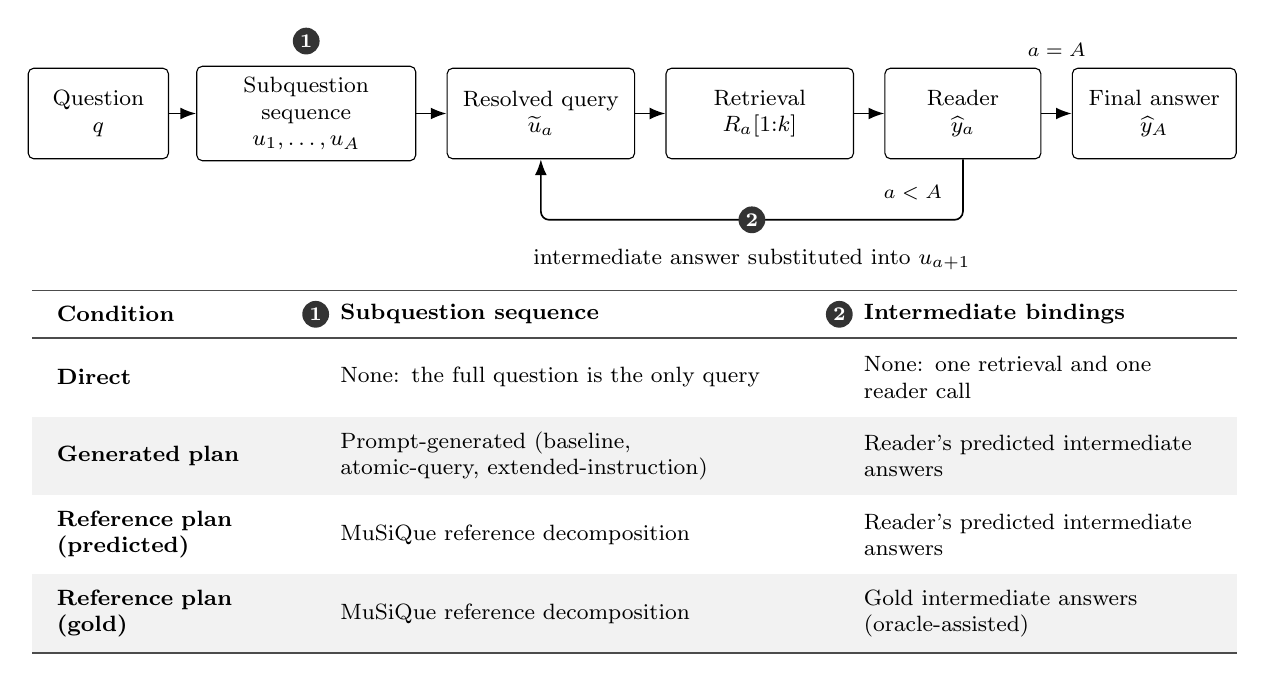
\begin{tikzpicture}[
      font=\footnotesize,
      box/.style={draw, rounded corners=2pt, align=center, inner sep=4pt,
                  minimum height=1.15cm,
                  execute at begin node={\hyphenpenalty=10000\exhyphenpenalty=10000}},
      flow/.style={-{Latex[length=2mm]}, semithick},
      back/.style={-{Latex[length=2mm]}, semithick, rounded corners=3pt},
      tag/.style={circle, fill=black!80, text=white, inner sep=0pt,
                  minimum size=3.4mm, font=\scriptsize\bfseries},
      cell/.style={anchor=west, align=left, inner sep=3pt,
                   execute at begin node={\hyphenpenalty=10000\exhyphenpenalty=10000}},
      rule/.style={draw=black!70, semithick}
    ]
    % --- Execution shared by every condition ---------------------------------
    \node[box, text width=1.5cm] (q)     at (-6.86,0)
      {Question\\\(q\)};
    \node[box, text width=2.5cm] (plan)  at (-4.22,0)
      {Subquestion sequence\\\(u_1,\dots,u_A\)};
    \node[box, text width=2.1cm] (query) at (-1.24,0)
      {Resolved query\\\(\widetilde u_a\)};
    \node[box, text width=2.1cm] (retr)  at (1.54,0)
      {Retrieval\\\(R_a[1{:}k]\)};
    \node[box, text width=1.7cm] (read)  at (4.12,0)
      {Reader\\\(\widehat y_a\)};
    \node[box, text width=1.8cm] (final) at (6.55,0)
      {Final answer\\\(\widehat y_A\)};

    \draw[flow] (q) -- (plan);
    \draw[flow] (plan) -- (query);
    \draw[flow] (query) -- (retr);
    \draw[flow] (retr) -- (read);
    \draw[flow] (read) -- (final);
    \node[font=\scriptsize, anchor=south] at (5.31,0.60) {\(a=A\)};

    % Sequential dependency: an earlier answer resolves a later subquestion.
    \draw[back] (read.south) -- (4.12,-1.35) -- (-1.24,-1.35) -- (query.south);
    \node[font=\scriptsize, anchor=east] at (3.98,-1.00) {\(a<A\)};
    \node[tag] at (1.44,-1.35) {2};
    \node[anchor=north, font=\footnotesize] at (1.44,-1.60)
      {intermediate answer substituted into \(u_{a+1}\)};

    \node[tag] at (-4.22,0.92) {1};

    % --- What each compared condition supplies at points 1 and 2 -------------
    \fill[black!5] (-7.70,-3.85) rectangle (7.60,-4.85);
    \fill[black!5] (-7.70,-5.85) rectangle (7.60,-6.85);

    \draw[rule] (-7.70,-2.25) -- (7.60,-2.25);
    \draw[rule] (-7.70,-2.85) -- (7.60,-2.85);
    \draw[rule] (-7.70,-6.85) -- (7.60,-6.85);

    \node[cell] at (-7.50,-2.55) {\textbf{Condition}};
    \node[tag]  at (-4.10,-2.55) {1};
    \node[cell] at (-3.90,-2.55) {\textbf{Subquestion sequence}};
    \node[tag]  at (2.55,-2.55) {2};
    \node[cell] at (2.75,-2.55) {\textbf{Intermediate bindings}};

    \node[cell, text width=2.8cm] at (-7.50,-3.35) {\textbf{Direct}};
    \node[cell, text width=6.2cm] at (-3.90,-3.35)
      {None: the full question is the only query};
    \node[cell, text width=4.3cm] at (2.75,-3.35)
      {None: one retrieval and one reader call};

    \node[cell, text width=2.8cm] at (-7.50,-4.35) {\textbf{Generated plan}};
    \node[cell, text width=6.2cm] at (-3.90,-4.35)
      {Prompt-generated (baseline,\\atomic-query, extended-instruction)};
    \node[cell, text width=4.3cm] at (2.75,-4.35)
      {Reader's predicted intermediate answers};

    \node[cell, text width=2.8cm] at (-7.50,-5.35)
      {\textbf{Reference plan}\\\textbf{(predicted)}};
    \node[cell, text width=6.2cm] at (-3.90,-5.35)
      {MuSiQue reference decomposition};
    \node[cell, text width=4.3cm] at (2.75,-5.35)
      {Reader's predicted intermediate answers};

    \node[cell, text width=2.8cm] at (-7.50,-6.35)
      {\textbf{Reference plan}\\\textbf{(gold)}};
    \node[cell, text width=6.2cm] at (-3.90,-6.35)
      {MuSiQue reference decomposition};
    \node[cell, text width=4.3cm] at (2.75,-6.35)
      {Gold intermediate answers (oracle-assisted)};
  \end{tikzpicture}
  \caption{Execution conditions in the retrieval study. The diagram is the
    execution shared by every condition, with the two marked points that the
    comparison varies: the source of the subquestion sequence and the source
    of the intermediate answers substituted into later subquestions. The
    table states what each condition supplies at those two points. Direct
    execution has neither, and the gold-binding condition is oracle-assisted.}
  \label{fig:ch4-execution-conditions}
\end{figure}

\paragraph{Measurements and comparisons.}

% TODO (before submission): the normalisation rules and the alias source below
% state what the evaluation script does. Confirm against the script itself.
Answer quality is measured by exact match (EM) and token F1 against the
reference answer and its accepted aliases, under the benchmark's answer
normalisation: lowercasing, removal of articles and punctuation, and collapse
of whitespace \cite{trivedi2022musique}. Let $t(\cdot)$ denote the token
multiset of a normalised string, and let $\mathcal{A}(y)$ denote the reference
answer $y$ together with its accepted aliases. Then
\begin{equation}
  \mathrm{EM}(\widehat y,y)=\mathbf{1}\{\widehat y\in\mathcal{A}(y)\},
  \qquad
  \mathrm{F1}(\widehat y,y)=\max_{y'\in\mathcal{A}(y)}
    \frac{2\lvert t(\widehat y)\cap t(y')\rvert}
         {\lvert t(\widehat y)\rvert+\lvert t(y')\rvert},
  \label{eq:ch4-answer}
\end{equation}
where all compared strings are normalised and $\cap$ is the multiset
intersection. Both quantities are averaged over the panel; EM is reported as a
percentage and F1 on a $0$--$100$ scale.

Retrieval is measured by complete-evidence coverage
(Equation~\ref{eq:ch4-coverage}), union depth (Equation~\ref{eq:ch4-union})
and ownership-masked depth (Equation~\ref{eq:ch4-masked}), summarised by the
depth score $J_D$ of Equation~\ref{eq:ch4-credit}. The number of generated arms, retrieved passage
slots and recorded total model tokens describe resource use. A passage slot is
one passage delivered to one reader call. Per-arm passage counts therefore
charge duplicate passages again when they are sent to separate reader calls,
while unique passage counts describe the pooled collection. Recorded tokens are
the prompt and completion tokens of the decomposition and reading calls of a
question.

The reference-answer control records one token total across several execution
branches. Per-branch costs are therefore unavailable. Generated and direct runs
have separate recorded totals, which are reported per question.

Comparisons pair the same questions across configurations. Where intervals are
reported, they are percentile intervals from $10\,000$ paired question-level
bootstrap resamples. They describe variation within this development panel.
Several prompt and attribution configurations were examined on the panel, so
these intervals are descriptive rather than a correction for adaptive model
selection. The reference-style ownership control was kept separate from weight fitting
and threshold calibration; its role is a structured assignment control rather
than an evaluation of arbitrary generated plans.

\section{Ownership Validation and Decomposition Results}
\label{sec:ch4-results}

The experiments assess both the evaluation framework and the decompositions
it measures. Ownership recovery tests whether the estimator can reproduce
known evidence assignments. The retrieval and answer comparisons then compare 
generated decomposition with direct retrieval and examine how intermediate 
answers affect the resulting execution.

\subsection{Ownership Prediction Accuracy}

The ownership ensemble recovers the complete reference assignment on
$92$ of $100$ questions, with precision of $97.46\%$ and recall of $98.18\%$.
Table~\ref{tab:ch4-ownership} reports the detailed measurements. The model
recovers $269$ of $274$ reference owner cells and selects seven non-owner
cells. At the subquestion level, $264$ of $274$ arm rows are exact. These
results support automatic ownership measurement on the evaluated
reference-style plans.

\begin{table}[htbp]
\centering
\caption{Ownership prediction on the reference-style decomposition control.
Cell metrics use $814$ subquestion--passage pairs. Complete-mask agreement is
measured over the $100$ questions.}
\label{tab:ch4-ownership}
\begin{tabular}{lr}
\hline
Measurement & Value \\
\hline
True positives / false negatives & $269\,/\,5$ \\
False positives / true negatives & $7\,/\,533$ \\
Precision & $97.46\%$ \\
Recall & $98.18\%$ \\
Cell accuracy & $98.53\%$ \\
AUROC of mean model scores & $0.9977$ \\
Exact arm rows & $264/274$ \\
Exact question masks & $92/100$ \\
\hline
\end{tabular}
\end{table}

The cohort breakdown in Table~\ref{tab:ch4-cohorts} shows the distribution of
the twelve cell errors. Four-hop questions contain three of the five missed
owners. Because several cells belong to the same question, cell totals are
reported with their question counts rather than interpreted as independent
question outcomes.

\begin{table}[htbp]
\centering
\caption{Ownership errors by reference hop count. TP, FN, FP and TN count
individual cells, while $n$ counts questions.}
\label{tab:ch4-cohorts}
\begin{tabular}{lrrrrrr}
\hline
Reference hops & $n$ & Cells & TP & FN & FP & TN \\
\hline
2 & 48 & 192 & 95 & 1 & 4 & 92 \\
3 & 30 & 270 & 89 & 1 & 0 & 180 \\
4 & 22 & 352 & 85 & 3 & 3 & 261 \\
\hline
\end{tabular}
\end{table}

On the gold-answer retrieval traces, the exact reference mask yields complete
assigned-evidence coverage of $100\%$ at depth $200$ and a score of $86.47$.
Using the learned ownership mask gives $97\%$ coverage and a score of
$84.84$. This comparison isolates the effect of replacing the reference
assignment with its prediction on those fixed lists.

\subsection{Sensitivity to Ownership Predictions}

Ownership predictions determine which ranks enter the masked depth. Adding
an owner adds a retrieval requirement and can increase the depth. Removing
an owner can reduce it if another owner remains; removing the last owner of
a required passage instead makes the depth infinite. Assignment errors can
therefore move the score in either direction. To distinguish these changes
from retrieval improvements, the following comparison holds the ranked lists
fixed and varies only the ownership model.

Table~\ref{tab:ch4-masks} scores the same retrieval traces under two
attribution models: an earlier predictor built on a different feature set, and
the retained model of Section~\ref{sec:ch4-ownership}. The baseline generated
decomposition receives scores of $52.32$ and $72.19$ respectively. The analogous atomic-query values
are $52.81$ and $66.64$. These changes arise from the assigned cells, with the
passages and ranks held fixed. On the reference arms with gold bindings the two
models differ by $24.98$ points, while replacing the retained prediction with
the exact reference assignment changes the score by $1.63$. The masked-depth
measurement is therefore more sensitive to the choice of attribution model than
to the residual error of the retained one.

\begin{table}[htbp]
\centering
\caption{Masked-depth measurements under two attribution models on fixed
GPT-4o-mini retrieval traces. Coverage is complete assigned-evidence coverage
at $K=200$; score is $J_{D_M}$ from Equation~\ref{eq:ch4-credit}. The
passages and their ranks are identical across rows, so only the assigned cells
differ. The last row uses the exact reference assignment.}
\label{tab:ch4-masks}
\small
\begin{tabular}{llrr}
\hline
Decomposition & Attribution & Coverage (\%) & Score \\
\hline
Baseline & Earlier model & 78 & 52.32 \\
Baseline & Retained model & 87 & 72.19 \\
Atomic-query & Earlier model & 77 & 52.81 \\
Atomic-query & Retained model & 81 & 66.64 \\
Reference, gold bindings & Earlier model & 88 & 59.86 \\
Reference, gold bindings & Retained model & 97 & 84.84 \\
Reference, gold bindings & Reference assignment & 100 & 86.47 \\
\hline
\end{tabular}
\end{table}

The reference-style control supports the use of the retained predictor for
recovering known assignments. For generated arms, assignments can legitimately
be fused or shared. The score differences in Table~\ref{tab:ch4-masks}
therefore establish sensitivity to attribution rather than a labelled accuracy
comparison on generated plans. Absolute masked-depth values on generated decompositions
should therefore be interpreted as estimator-dependent diagnostics. Comparisons between 
prompts hold this source of variation fixed and are reported alongside ownership-independent 
union coverage and final-answer measurements.

\subsection{Decomposition versus Direct Retrieval}

For readability, $C_U(k)$ denotes the union coverage
$C_{D_{\mathrm{union}}}(k)$ in the result tables.
Table~\ref{tab:ch4-system} reports the direct and generated-decomposition
executions. With GPT-4o-mini, the baseline decomposition raises complete union
coverage at five passages per arm from $45\%$ to $76\%$. EM changes from
$40\%$ to $52\%$ and F1 from $52.64$ to $59.00$. With Llama-3.3-70B,
complete union coverage changes from $46\%$ to $79\%$, while EM changes from
$42\%$ to $43\%$ and F1 from $52.30$ to $51.37$.

\begin{table}[htbp]
\centering
\caption{Recorded execution results on $100$ MuSiQue questions. EM and F1
are percentages. $C_U(5)$ is complete union coverage at five passages per arm.
Arms and tokens are per-question means. Retrieved evidence and final answers
are separate outcomes.}
\label{tab:ch4-system}
\small
\begin{tabular}{llrrrrr}
\hline
Model & Prompt & EM & F1 & $C_U(5)$ & Arms & Tokens \\
\hline
GPT-4o-mini & Direct & 40 & 52.64 & 45 & 1.00 & 4\,369 \\
 & Baseline & 52 & 59.00 & 76 & 2.79 & 12\,763 \\
 & Atomic-query & 52 & 59.66 & 72 & 2.66 & 11\,898 \\
 & Extended-instruction & 50 & 60.39 & 74 & 2.61 & 13\,881 \\
\hline
Llama-3.3-70B & Direct & 42 & 52.30 & 46 & 1.00 & 4\,530 \\
 & Baseline & 43 & 51.37 & 79 & 3.00 & 14\,069 \\
 & Atomic-query & 45 & 53.54 & 78 & 3.22 & 14\,789 \\
 & Extended-instruction & 47 & 55.94 & 75 & 2.84 & 15\,271 \\
\hline
\end{tabular}
\end{table}

The paired bootstrap interval for the baseline decomposition's EM change is
$[2,22]$ percentage points for GPT-4o-mini and $[-8,10]$ for Llama-3.3-70B.
On this 100-question development panel, the GPT-4o-mini decomposition is associated 
with higher answer accuracy as well as higher evidence coverage. This end-to-end comparison 
is not compute-matched, since decomposition uses additional passage slots and reader calls; 
Section 4.6 isolates retrieval behaviour under a matched passage-slot budget.
The Llama result shows that increased evidence coverage does not necessarily translate into a 
comparable answer-quality gain, motivating the controlled intermediate-answer experiment below.

The per-arm comparison also changes the total retrieval expenditure. The
baseline GPT-4o-mini decomposition retrieves a mean of $13.95$ passage slots
across its reader calls, compared with $5$ for direct retrieval. Its mean pooled
collection contains $11.35$ distinct passages. Thus the coverage increase in
Table~\ref{tab:ch4-system} combines a change in query formulation with more
passage slots and more reader calls. Section~\ref{sec:ch4-budget} compares
fixed lists at a common total passage budget.

\subsection{The Effect of Intermediate Answers}

The two reference-decomposition controls use the same subquestion templates
and reader but change the answers substituted into later queries.
Table~\ref{tab:ch4-bindings} reports their outcomes. Gold substitution yields
EM $64\%$ versus $49\%$ under predicted substitution, with a paired bootstrap
interval of $[8,22]$ percentage points for the difference. Complete union
coverage at five passages per arm changes from $80\%$ to $92\%$.

\begin{table}[htbp]
\centering
\caption{Reference-decomposition controls with GPT-4o-mini. Gold bindings
supply reference intermediate answers when constructing downstream queries.
Predicted bindings use the reader's earlier outputs.}
\label{tab:ch4-bindings}
\begin{tabular}{lrrr}
\hline
Intermediate substitution & EM (\%) & F1 & $C_U(5)$ (\%) \\
\hline
Predicted answers & 49 & 57.50 & 80 \\
Gold answers & 64 & 70.73 & 92 \\
\hline
\end{tabular}
\end{table}

The control identifies intermediate answers as a point of intervention in the
retrieval chain. Correct substitutions improve downstream query text and the
evidence available for answering. Because this experiment supplies gold
answers, it measures the benefit of correcting intermediate state within the
reference pipeline. This finding motivates recording intermediate predictions
alongside retrieval outcomes when constructing optimisation feedback.

\paragraph{Reference and generated queries with BM25.}
A complementary MuSiQue comparison examines reference plans with gold
intermediate answers and generated plans with predicted answers under BM25.
Both search the same $11\,656$-passage corpus. Generated traces use five
passages per intermediate reader call, and each ranked list is saved to depth
$200$. Table~\ref{tab:ch4-bm25-regimes} reports complete-evidence coverage
when a total budget of $8$ or $200$ passage slots is divided as evenly as
possible across the subquestions. Section~\ref{sec:ch4-budget} defines this
allocation formally, and Section~\ref{sec:ch4-bm25} gives the BM25 panel
and trace-generation details.

\begin{table}[H]
\centering
\small
\caption{MuSiQue BM25 retrieval regimes. Coverage (\%) is measured on each
retained panel under balanced slot allocation at total budgets $B=8$ and
$B=200$. The reference row uses a different plan source and a larger panel.}
\label{tab:ch4-bm25-regimes}
\begin{tabular}{lrrr}
\hline
Query regime & $n$ & $B=8$ & $B=200$ \\
\hline
Reference plan, gold bindings & $1\,000$ & $59.5$ & $96.2$ \\
Generated plan, predicted bindings & $824$ & $41.3$ & $73.3$ \\
\hline
\end{tabular}
\end{table}

The reference regime achieves higher coverage at both budgets, reaching
$96.2\%$ at $B=200$, compared with $73.3\%$ for generated plans.
This is a descriptive, oracle-assisted comparison: both the plan source
and the intermediate answers change, and the panels contain $1\,000$
reference questions and $824$ retained generated traces. The gap therefore
cannot be attributed to intermediate-answer quality alone. The controlled
reference-chain experiment above isolates that change while holding the
subquestion templates fixed.

\section{Evidence Coverage Under a Passage Budget}
\label{sec:ch4-budget}

The evidence-rank framework also makes it possible to study how passages
should be distributed across subquestions. We compare a balanced allocation
with a gold-informed oracle under the same total passage budget, holding
the recorded queries fixed. The resulting coverage gap quantifies the
opportunity for a learned allocator. We evaluate it first on the original
MuSiQue panel and then with BM25 across three benchmarks.

\subsection{Passage-Slot Accounting and Balanced Allocation}

A common per-arm depth gives more total passage slots to longer decompositions.
To compare questions under the same total allowance, consider a per-question
ceiling $B\leq AK$ distributed among the $A$ recorded retrieval lists.
Balanced allocation uses the whole allowance and assigns
\begin{equation}
  k_a(B)=\left\lfloor\frac{B}{A}\right\rfloor
        +\mathbf{1}\{a\leq B\bmod A\},
  \qquad
  \sum_{a=1}^{A}k_a(B)=B.
  \label{eq:ch4-budget-allocation}
\end{equation}
The remainder is allocated in execution order. For example, a budget of
eight slots shared by three arms gives depths $(3,3,2)$. Each occurrence
of a passage in a selected prefix costs one slot, including duplicates across
arms. Complete evidence availability is evaluated in the pooled set
$\bigcup_a R_a[1:k_a(B)]$; no ownership mask is needed for this union criterion.

This allowance counts selected passage slots. The same number of slots can produce
different numbers of unique passages and different token totals, since passages
can recur across arms and vary in length. Retrieving the ranked lists, producing
the queries and reading the contexts incur separate computational costs.

These are fixed-list replays. The original intermediate answers and later
queries were generated using five passages per reader call. Changing a prefix
in the replay leaves those earlier answers and later queries unchanged. The
result measures the coverage of the recorded lists at a specified slot budget.
An end-to-end policy evaluated at that budget would regenerate intermediate
answers and dependent queries under its actual contexts.

The ceiling applies to each question separately. Its largest feasible common
depth is $\lfloor B/A(q)\rfloor$, with the balanced rule also spending the
remainder. A single depth shared across the panel would be limited by the
longest plan to $\lfloor B/\max_q A(q)\rfloor$, leaving slots unused for
shorter plans. Allowing transfers between questions under an average budget
would define a different allocation problem.

\subsection{Oracle Allocation on Recorded Lists}

Supporting passages need not occur at similar ranks across arms. For example,
if two arms contain distinct required passages at ranks two and six, with
neither passage available elsewhere, a balanced $(4,4)$ allocation misses
one passage whereas $(2,6)$ covers both at the same cost. The oracle uses
gold evidence identities to find the least expensive prefix allocation that
covers a question:
\begin{equation}
  B^*(q)=
  \min_{k_1,\ldots,k_A\in\{0,\ldots,K\}}
  \left\{\sum_a k_a:
    E(q)\subseteq\bigcup_a R_a[1:k_a]
  \right\}.
  \label{eq:ch4-oracle-budget}
\end{equation}
The value is $+\infty$ when the retained lists jointly miss annotated
evidence. For finite cases, it can be computed by dynamic programming over
subsets of evidence. Let $S_a(k)$ denote the evidence indices found in arm
$a$'s first $k$ passages. Starting from $F_0(\varnothing)=0$, the update is
\begin{equation}
  F_a(T\cup S_a(k))
  \leftarrow
  \min\{F_a(T\cup S_a(k)),F_{a-1}(T)+k\}.
  \label{eq:ch4-dynamic-program}
\end{equation}
Unreachable states have value $+\infty$, and
$B^*(q)=F_A(\{1,\ldots,h\})$. Only zero and prefix lengths at which an
additional evidence item appears need to be considered: a longer prefix with
the same evidence set adds cost without changing that state. With at most
four annotated hops in these experiments, the subset state space is small.

The oracle uses gold evidence identities to choose its allocation. Moreover,
all recorded queries are available even when their selected prefix length is
zero. The objective charges passage slots but leaves the generation of those
queries and their intermediate states outside the optimisation. It is an exact
minimum for the fixed-list problem and an optimistic reference for a system
that must construct and execute the queries. It is not an achieved runtime or
token saving.

Applying the coverage aggregation in Equation~\ref{eq:ch4-coverage} to
these minimum budgets gives the oracle coverage frontier:
\begin{equation}
  C^*(B)=\frac{1}{n}\sum_{q=1}^{n}
  \mathbf{1}\{B^*(q)\leq B\}.
  \label{eq:ch4-oracle-frontier}
\end{equation}
It is the fraction of questions whose complete evidence can be recovered
within $B$ slots under the best prefix allocation. A question missing a
required passage from every saved list remains uncovered at every budget.

\subsection{Allocation Results on the MuSiQue Panel}
\label{sec:ch4-musique-budget}

The replay uses the same $100$ MuSiQue questions and HippoRAG~2 rankings as
the execution study. Its budget of $B=15$ is close to the baseline
GPT-4o-mini decomposition's mean of $13.95$ passage slots, giving the
comparison a similar selected-passage allowance. At $B=15$, balanced allocation
recovers complete evidence for $76$ questions under the baseline GPT-4o-mini
decomposition and $78$ under its Llama counterpart. The corresponding oracle
allocations reach $85$ and $87$; an oracle entry counts the questions whose
minimum feasible budget $B^*(q)$ in Equation~\ref{eq:ch4-oracle-budget} is at
most $15$. Table~\ref{tab:ch4-budget} reports the same comparison for the
other prompts and for direct retrieval, which are the configurations available
without a reference decomposition. Direct retrieval has a single arm, so its
two allocations coincide by construction, and its entries give that one list
$15$ passages rather than the five used in execution.

\begin{table}[htbp]
\centering
\caption{Complete evidence coverage (\%) at a total budget of $15$ passage
slots on fixed recorded lists. The oracle chooses prefixes using gold evidence
and is a reference allocation rather than a deployed policy. Each row contains
$100$ questions.}
\label{tab:ch4-budget}
\begin{tabular}{llrr}
\hline
Model & Prompt & Balanced allocation & Oracle allocation \\
\hline
GPT-4o-mini & Direct & 66 & 66 \\
 & Baseline & 76 & 85 \\
 & Atomic-query & 73 & 85 \\
 & Extended-instruction & 75 & 83 \\
\hline
Llama-3.3-70B & Direct & 65 & 65 \\
 & Baseline & 78 & 87 \\
 & Atomic-query & 75 & 88 \\
 & Extended-instruction & 75 & 85 \\
\hline
\end{tabular}
\end{table}

On these fixed recorded rankings, the baseline decompositions retain a complete-evidence 
coverage advantage over direct retrieval after matching the total selected passage-slot budget. 
The additional nine questions recoverable by oracle allocation on the baseline decomposition in
each model setting show that redistributing slots can recover evidence missed
by the balanced split. This provides a concrete target for the learned policies in
Chapter~5: recover more supporting evidence by choosing depths from
observable query and retrieval features.

\subsection{Cross-Benchmark BM25 Evaluation}
\label{sec:ch4-bm25}

The next study examines whether the allocation opportunity also appears with
a different retriever and on other datasets. It uses BM25 over separate
closed corpora containing $11\,656$ passages for MuSiQue, $10\,426$ for
2WikiMultiHopQA~\cite{ho2020constructing}, and $9\,811$ for
HotpotQA~\cite{yang2018hotpotqa}. The MuSiQue corpus is unchanged from the
earlier experiment; the question panel is larger.

\paragraph{Evaluation population and trace generation.}
Each source panel contains $1\,000$ questions. Within the available compute
budget, trace generation retained $824$ MuSiQue, $977$ 2WikiMultiHopQA,
and $996$ HotpotQA questions. All allocation comparisons and the
full-question control use the same retained IDs within each benchmark.
Retention follows execution order and per-question cost, not retrieval or
answer outcomes. Coverage therefore describes the retained questions. These
panels also informed development and are separate from the frozen comparison
in Chapter~5.

Generated subquestions are executed sequentially with GPT-4o-mini. Each
retrieval call searches the full benchmark corpus, the reader receives the
top five passages, and its predicted answer resolves references in later
subquestions. The top $200$ passages from each ranked list are saved.
Allocation uses these fixed lists and the passage-slot accounting defined
above, preserving the answers and queries produced during trace generation.

\paragraph{Coverage at a matched budget.}
Table~\ref{tab:ch4-bm25-availability} compares full-question retrieval,
balanced allocation, and the oracle at $B=8$. Full-question retrieval
selects eight passages from its single list. Balanced allocation divides
the same budget among the generated subquestions, while the oracle chooses
their prefix lengths using gold evidence ranks. The recorded plans contain
at most seven arms on MuSiQue and HotpotQA and six on 2Wiki, so balanced
allocation can give every arm at least one slot.

\begin{table}[htbp]
\centering
\small
\caption{Complete annotated-evidence coverage at a ceiling of eight selected passage slots. BM25 results use fixed predicted-binding traces; the oracle uses gold evidence ranks. Counts are retained questions from each original 1,000-question panel.}
\label{tab:ch4-bm25-availability}
\begin{tabular}{lrrrr}
\hline
Dataset & $n$ & Full question & Balanced & Oracle \\
\hline
MuSiQue & 824 & 0.136 & 0.413 & 0.536 \\
2Wiki & 977 & 0.315 & 0.688 & 0.881 \\
HotpotQA & 996 & 0.637 & 0.762 & 0.836 \\
\hline
\end{tabular}
\end{table}


On the retained fixed traces, balanced allocation achieves higher complete
annotated-evidence coverage than full-question retrieval at \(B=8\) on all
three benchmarks, while the gold-informed oracle provides additional headroom. 
On MuSiQue, for example,
coverage rises from $13.6\%$ with full-question retrieval to
$41.3\%$ with balanced allocation and $53.6\%$ with the oracle.
The gap between balanced and oracle allocation shows the
opportunity to improve coverage by distributing the same
passage budget unevenly across arms. Some lists require deeper
prefixes to reach supporting evidence, while others can
contribute their evidence with fewer slots. This allocation
headroom therefore also appears with BM25 and across all three
benchmarks.

The dynamic program in Equation~\ref{eq:ch4-dynamic-program}
independently reproduces the saved oracle coverage on all three panels at
the checked budgets.

\paragraph{Budgets needed for target coverage.}
The same comparison can be read in terms of the budget needed
to reach a coverage target. On the MuSiQue sequential panel,
balanced allocation first reaches $50\%$, $60\%$, and $70\%$
coverage at $16$, $32$, and $128$ slots, respectively. The
oracle reaches these targets at $8$, $16$, and $48$ slots.
These are the first tested budgets that meet each target,
rather than exact minimum budgets over all possible values.

At $B=200$, the MuSiQue oracle reaches $79.5\%$ coverage, compared with
$73.3\%$ under balanced allocation. This comparison uses the generated
regime from Table~\ref{tab:ch4-bm25-regimes}. The remaining oracle gap
concerns redistribution within the saved lists. Improving the queries or
changing the intermediate reader contexts would require new execution;
neither effect is measured by this replay.

Finally, allocation depends on the number of generated arms,
whose means are $2.53$, $2.79$, and $2.10$ on MuSiQue, 2Wiki,
and HotpotQA, respectively. More arms provide more allocation
choices, but may also reflect redundant splitting or prompt
preferences. Any association between arm count and allocation
headroom therefore concerns the generated plan structure;
it does not by itself show that harder questions offer
greater savings.

\section{Discussion and Implications for Optimisation}
\label{sec:ch4-discussion}

\subsection{Contributions and Implications}

The framework links evidence responsibility to retrieval depth. Ownership
assignments distinguish pooled evidence availability from retrieval by the
intended subquestion, complementing final-answer measurements.

On the 100-question MuSiQue development panel, generated decomposition increases 
evidence coverage under both reader settings and is associated with higher 
final-answer accuracy for GPT-4o-mini. Because the end-to-end comparison uses 
more passage slots and reader calls, the separate fixed-list replay evaluates 
retrieval under matched passage-slot budgets. Matched-budget replay shows that redistributing passage
slots can recover evidence missed by balanced allocation, an opportunity
also observed with BM25 across three benchmarks.

Chapter~5 applies these foundations: the ownership-masked score evaluates
OPRO candidates, the oracle frontier motivates learned allocation, and the
execution diagnostics structure feedback for prompt revision.

\subsection{Scope and Limitations}
\label{sec:ch4-limitations}

Ownership validation uses reference-style decompositions with known supporting
passages. Its archived template history is only partially documented, and
accuracy on naturally generated plans requires independently labelled
assignments. The estimator assigns a supplied evidence set; discovering that
set for a new question is a separate task. Its threshold and voting procedure
are assessed empirically, with simultaneous assignment guarantees requiring
additional assumptions.

The retrieval comparisons describe development panels under the reported
models and corpus scope. Bootstrap intervals measure variation within those
panels. The reference-versus-generated BM25 comparison changes both the plans
and intermediate answers on different populations, so the controlled
reference-chain experiment provides the narrower evidence about substitution.
Per-branch token costs are also unavailable for the reference-answer controls.

Allocation replay preserves queries generated with five passages per
intermediate reader call. Its budget counts selected slots, including repeated
passages, and excludes trace generation. Oracle improvements therefore
quantify the potential of the saved rankings. Measuring operational savings
requires a policy evaluated with its actual reader contexts, answer quality,
and execution cost.

\section*{Conclusion}

This chapter connected retrieval ranks to learned evidence ownership,
recovering $92$ of $100$ complete reference-style masks. On the MuSiQue
panel, decomposition improved evidence retrieval and raised GPT-4o-mini
exact match from $40\%$ to $52\%$. Intermediate-answer controls further
showed why plan execution matters alongside evidence availability.

Gold-informed oracle allocation further showed, across three BM25 benchmarks, 
that unequal allocation can recover supporting evidence missed by a balanced split, 
establishing the headroom studied by the learned allocator in Chapter 5. 
Chapter~5 turns these measurements and diagnostics into
tools for prompt search and passage selection.

\chapter{Optimising Question Decomposition and Evidence Allocation}
\label{chap:optimisation}

\section*{Introduction}

Chapter~4 introduced an evidence-aware evaluation of a generated decomposition.
The ownership mask assigns supporting passages to subquestions, and the resulting
depth score measures how early those passages can be retrieved by their assigned
queries. This chapter uses that score to optimise the instruction that generates
the decomposition. It addresses the question posed in Section~2.6.2: can the
generation strategy preserve evidence coverage while reducing retrieval depth?

The completed experiment applies an OPRO-style search to one system instruction.
It evaluates twenty-four proposed instructions and the initial instruction on
the same hundred MuSiQue questions. The selected instruction raises the masked
depth score from $66.30$ to $67.20$, with unchanged exact match of $44\%$.
These measurements describe prompt selection on the development panel. They
also motivate a distinction between improving a retrieval objective and
improving the answers produced by the complete system.

The chapter presents two complementary interventions. Prompt search changes
the questions issued by the system. Learned allocation changes the passage
prefix selected from each arm of a recorded execution. The completed allocation
study uses predicted-binding BM25 traces on MuSiQue, 2Wiki and HotpotQA. At a
budget of eight passage slots, its largest observed coverage increase is
$6.3$ percentage points on 2Wiki. These are retrieval-coverage measurements
on retained traces, distinct from the pilot's final-answer measurements.
A paired $700$-question MuSiQue experiment also evaluates the answers
produced from balanced and segment-policy pooled contexts. The later
unit-increment policy is evaluated separately on retrieval coverage.

The chapter then specifies an evidence-feedback extension that separates observed retrieval
and dependency information from estimated ownership. A comparison with
answer-only and information-matched raw feedback is defined on frozen
optimisation, selection and confirmation splits. The extension has an
implemented feedback and search interface; its comparative answer-quality
evaluation remains prospective. The empirical conclusions concern the
completed OPRO pilot, fixed-trace allocation study and controlled ownership
stress tests.

\section{The Optimisation Problem}

\subsection{An Instruction Defines an Executable Policy}

Let $p$ denote the decomposer's system instruction and let $q$ be an input
question. With fixed demonstrations and generation settings, the decomposer
produces an ordered plan
\begin{equation}
  \pi_p(q)=(u_1,\ldots,u_{A_p(q)}),
  \label{eq:ch5-plan}
\end{equation}
where $A_p(q)$ is the number of subquestions. A reference \texttt{\#i} in
$u_a$ refers to the answer of an earlier arm, so valid references satisfy
$i<a$. The executor substitutes its predicted intermediate answers, retrieves
passages and reads them for each arm in sequence. The answer of the last arm
is the final answer $\widehat y_p(q)$.

This interface constrains useful prompt changes. Each arm must be phrased as a
retrieval question, references must be executable in order, and the final arm
must target the answer requested by $q$. A plan that retrieves relevant facts
but ends with an intermediate entity can have adequate evidence coverage and
an incorrect final answer. The optimisation therefore acts on a program of
retrieval and reading steps, rather than on a list of paraphrases alone.

The historical experiment changes $p$ while keeping the demonstrations,
retriever, reader and ownership estimator fixed. It uses one generated plan
per question. The six instructions proposed in a search round are six policy
candidates, not six plans combined at inference time.

\subsection{The Retained Retrieval Objective}

For each executed plan, let $D_{M,p}(q)$ be the ownership-masked depth defined
in Chapter~4. It is the greatest passage rank among the assigned arm--evidence
pairs, with infinite depth when required evidence has no predicted owner or
falls outside the retained ranked lists. With cutoff $K=200$, the search
objective is
\begin{equation}
  J_M(p;\mathcal D)=\frac{100}{|\mathcal D|}
       \sum_{q\in\mathcal D}v_K\!\left(D_{M,p}(q)\right),
  \qquad
  v_K(d)=
  \begin{cases}
     1-\dfrac{\log d}{\log K},&1\leq d\leq K,\\[1mm]
     0,&d=+\infty.
  \end{cases}
  \label{eq:ch5-objective}
\end{equation}
All questions remain in the denominator. The objective rewards early complete
retrieval under the predicted assignment and gives zero credit to a censored
question. Its companion coverage statistic is
\begin{equation}
  C_M(K;p)=\frac{1}{|\mathcal D|}\sum_{q\in\mathcal D}
             \mathbf{1}\{D_{M,p}(q)\leq K\}.
  \label{eq:ch5-coverage}
\end{equation}
Depth $K$ receives zero logarithmic credit but counts as finite coverage.
Reporting both quantities distinguishes complete evidence near the search
limit from incomplete evidence.

The score depends on the ownership estimator. An assignment error can change
which ranks enter the maximum, as discussed in Chapter~4. The estimator is
therefore frozen during search. Evidence coverage computed directly from the
gold passage set remains a separate diagnostic.

\subsection{Answer Quality and Resource Use}

The end-to-end outcomes are exact match and token F1 against the benchmark
reference answers. For a fixed evaluation panel, define
\begin{equation}
  J_{\mathrm{F1}}(p)=\frac{1}{|\mathcal D|}
       \sum_{q\in\mathcal D}\mathrm{F1}(\widehat y_p(q),y_q).
  \label{eq:ch5-f1}
\end{equation}
The retrieval objective in Equation~\ref{eq:ch5-objective} and the answer
objective in Equation~\ref{eq:ch5-f1} measure different properties. Retrieved
evidence must still be read, intermediate answers must bind correctly, and the
last arm must produce the requested answer.

The historical reader consumes five passages per arm. Its nominal passage-slot
allowance is consequently $5A_p(q)$, with repeated passages charged to each
arm that reads them. Unique passages, reader tokens and model calls are
additional cost measurements. The masked-depth objective contains no direct
penalty for arm count, so a higher objective value alone establishes neither
lower total reading cost nor higher answer accuracy.

\section{The Completed OPRO Search}

\subsection{Search Configuration}

OPRO uses a language model to propose solutions from a history of candidates
and their measured scores~\cite{ch5-opro}. Here, a candidate is the text of
the decomposer's system instruction. GPT-4o proposes instructions, and the
Llama-3.3-70B pipeline executes them on the development questions.
Table~\ref{tab:ch5-configuration} records the retained configuration.

\begin{table}[tbp]
\centering
\small
\caption{Configuration of the completed prompt-search pilot.}
\label{tab:ch5-configuration}
\begin{tabular}{p{0.36\textwidth}p{0.55\textwidth}}
\hline
Component & Setting \\
\hline
Evaluation panel & The same $100$ MuSiQue questions for every candidate \\
Initialisations & One initial instruction \\
Search rounds & Four, with six new instructions per round \\
Candidate total & $25$, including the initial instruction \\
Proposal model & GPT-4o, temperature $1.0$ \\
Execution model & Llama-3.3-70B, one plan per question \\
Reader context & Five passages per executed arm \\
Retrieval scoring & Up to $200$ retained ranks per arm \\
Search reward & Ownership-masked logarithmic depth score \\
History in feedback & At most $20$ prior instructions and their rounded scores \\
Example feedback & Three cases from the current leading instruction \\
\hline
\end{tabular}
\end{table}

The executor uses temperature-zero generation with cached model calls. Exact
duplicate instruction hashes are filtered. The retained leaderboard contains
twenty-five successfully evaluated candidates and zero rejected candidates.
This amounts to $2\,500$ candidate--question evaluations. That count describes
logical evaluations; cached calls can reduce the number of billable model
requests.

The baseline is the seed instruction and its executions recorded within this
search. The separately recorded prompt variants in Chapter~4 provide context
for the pipeline, rather than substituting for this paired baseline.

\subsection{Proposal and Selection Loop}

The search begins by executing the initial instruction on all hundred
questions. At each round, the optimizer receives the retained instruction
history, the corresponding aggregate depth scores and three examples from
the current leader. It proposes six replacement instructions. Each is
executed through the same retrieval and reading pipeline, assigned an
ownership mask and scored using Equation~\ref{eq:ch5-objective}. The updated
leaderboard retains the highest-scoring instruction across all completed
rounds.

The full-precision score determines the leaderboard order, while the
meta-prompt displays integer-rounded scores. Twelve of the twenty-five
candidates are displayed in the same score-$64$ bucket. This reduces the
resolution of the numerical information available to the proposer, even
though their stored scores remain distinct.

The initial and selected instructions share the same planning policy: use
complete natural-language questions, preserve independent branches, require
backward references and split compound lookups into simpler arms. The selected
instruction adds an explicit check that the necessary facts of the original
question are covered. These are observed differences in instruction text.
The experiment changes several clauses together, so the measured score change
cannot be assigned to that coverage clause alone.

\subsection{The Feedback Supplied to the Optimizer}

The historical feedback prioritises questions with predicted unowned
evidence, then questions with the greatest masked depth. It selects the
unowned cases in stored question order. This gives the optimizer examples of
poorly scored executions, but repeatedly drawing from the current leader and
a fixed ordering can concentrate attention on a small part of the panel.

The example description attributes failures to facts that the plan failed to
ask for. That interpretation is stronger than the underlying measurements.
A passage may be assigned to an appropriate query yet appear at a large
retrieval rank. Conversely, an unowned passage is an estimator output whose
correctness depends on the ownership model. Both cases can lower the depth
score, while suggesting different changes to the instruction. This motivates
the typed feedback in Section~\ref{sec:ch5-feedback}.

\section{Results of the Pilot}

\subsection{Progress Across Search Rounds}

Table~\ref{tab:ch5-rounds} separates the best proposal in each round from the
best instruction retained so far. The overall winner appears in the second
round. The third and fourth rounds produce lower-scoring candidates, while
the stored best score remains $67.20$.

\begin{table}[tbp]
\centering
\caption{Masked-depth score during the completed search. The retained best
includes all earlier rounds. Values are on the shared development panel.}
\label{tab:ch5-rounds}
\begin{tabular}{lrrr}
\hline
Stage & New candidates & Best in stage & Retained best \\
\hline
Initial instruction & $1$ & $66.3017$ & $66.3017$ \\
Round $1$ & $6$ & $66.5975$ & $66.5975$ \\
Round $2$ & $6$ & $67.2042$ & $67.2042$ \\
Round $3$ & $6$ & $65.2557$ & $67.2042$ \\
Round $4$ & $6$ & $66.0482$ & $67.2042$ \\
\hline
\end{tabular}
\end{table}

The increase from the initial instruction is $0.9025$ score points. A plateau
over the final two rounds describes this trajectory and its proposal budget.
Broader search, different initial instructions and alternative feedback are
separate experimental choices. The four-round trajectory does not determine
their attainable performance.

\subsection{The Selected Instruction}

Table~\ref{tab:ch5-selected} compares the selected instruction with the seed
on the quantities available for both. Finite masked coverage remains at
$80\%$. Thus the higher aggregate score is not accompanied by a higher
aggregate count of questions with finite masked depth. Question-level
successes can still change identity.

\begin{table}[tbp]
\centering
\small
\caption{Initial and selected instructions on the $100$ development
questions. F1 is displayed on a $0$--$100$ scale. Passage slots are the
five-per-arm allowance derived from the observed arm count.}
\label{tab:ch5-selected}
\begin{tabular}{lrrr}
\hline
Measurement & Initial & Selected & Change \\
\hline
Masked-depth score & $66.3017$ & $67.2042$ & $+0.9025$ \\
Finite masked coverage (\%) & $80$ & $80$ & $0$ \\
Exact match (\%) & $44$ & $44$ & $0$ \\
Token F1 & $52.3682$ & $52.4847$ & $+0.1165$ \\
Mean generated arms & $3.00$ & $3.13$ & $+0.13$ \\
Mean passage-slot allowance & $15.00$ & $15.65$ & $+0.65$ \\
\hline
\end{tabular}
\end{table}

Exact match is unchanged at $44\%$: two questions change from incorrect to
correct and two change in the opposite direction. Mean F1 increases by
$0.1165$ points on the $0$--$100$ scale. The selected instruction generates
$0.13$ additional arms per question, corresponding to a $4.3\%$ increase in
the mean passage-slot allowance. Its measured benefit is therefore specific
to the masked-depth score, with broadly similar final-answer quality and a
slightly larger nominal reading allowance.

A paired bootstrap over the hundred questions gives a descriptive $95\%$
interval of $[-1.80,3.90]$ points for the masked-depth-score difference and
$[-3.60,4.00]$ points for the F1 difference. The exact-match difference has
an interval of $[-4,4]$ percentage points. These intervals condition on the
selected pair of instructions. The same panel supplied feedback and selected
the winner, so the intervals describe sensitivity to the sampled questions;
they are not an independent assessment of selection generalisation.

\subsection{The Optimisation Objective and the Answer Objective}

Across the twenty-five evaluated instructions, the Spearman correlation
between masked-depth score and mean answer F1 is $0.413$. The candidates are
adaptively related and share their evaluation questions, so this is a
description of the retained candidate set. It is useful for inspecting
whether the objective ranks these instructions like answer quality does.

The highest-F1 candidate occurs in the third round. It achieves F1 $53.88$
and exact match $46\%$, with masked-depth score $64.10$. The depth-selected
winner has F1 $52.48$ and exact match $44\%$, with score $67.20$.
Table~\ref{tab:ch5-objectives} shows the resulting reversal. The highest-F1
candidate is a retrospective comparator, not a second independently selected
test winner.

\begin{table}[tbp]
\centering
\small
\caption{Different objectives select different candidates from the same
development search. The F1-leading candidate is identified retrospectively.}
\label{tab:ch5-objectives}
\begin{tabular}{lrrr}
\hline
Instruction & Depth score & F1 & Exact match (\%) \\
\hline
Initial & $66.30$ & $52.37$ & $44$ \\
Highest depth score & $67.20$ & $52.48$ & $44$ \\
Highest answer F1 & $64.10$ & $53.88$ & $46$ \\
\hline
\end{tabular}
\end{table}

This result supports reporting retrieval quality and answer quality together.
An evidence-depth objective remains appropriate when the task is to bring
assigned evidence earlier in the ranked lists. For a claim about improved
question answering, final answers provide the direct selection criterion.
Objective choice and feedback choice should therefore be varied separately.

\section{Learned Allocation on Fixed Retrieval Traces}
\label{sec:ch5-allocation}

\subsection{The Allocation Intervention}

Prompt optimisation changes a plan and its resulting rankings. Allocation
holds those rankings fixed and chooses how much evidence to retain from each
arm. For a question with $A$ recorded arms, let $k_a$ be the prefix length
selected from arm $a$. Its passage-slot budget is
\begin{equation}
  \sum_{a=1}^{A}k_a\leq B.
  \label{eq:ch5-slot-budget}
\end{equation}
Complete coverage means that every annotated supporting passage occurs in
at least one selected prefix. This is the union criterion from Chapter~4.
An occurrence in two arms is charged twice in Equation~\ref{eq:ch5-slot-budget},
although a pooled reader may later deduplicate it.

The learned policy is evaluated on BM25 rankings generated by a sequential
execution. Each subquestion is answered using its first five retrieved
passages; that predicted answer resolves references in later subquestions.
The run retains $200$ ranks per arm. Allocation replays these saved lists.
Changing $B$ therefore preserves the intermediate answers and downstream
queries from the five-passages-per-hop trace-generation policy. The experiment
measures context selection conditional on that policy, rather than a fresh
budget-dependent execution of the reasoning chain.

The balanced comparator assigns $\lfloor B/A\rfloor$ slots to every arm and
distributes the remainder to the earliest arms. The learned rule also starts
with one slot per arm. Both comparisons use the same total budget when
$B\geq A$. The retained traces contain at most seven arms, so the budgets
$8$, $16$ and $32$ reported below satisfy that condition. Zero-depth arms
are allowed in the gold-informed oracle from Chapter~4; it is a reference
with a broader feasible set than these floor-constrained policies.

\subsection{Predicting Per-Arm Depth Requirements}

Training assigns each supporting passage to the arm that ranks it earliest,
breaking ties by arm order. An arm's target depth $d_a$ is the largest rank
among its assigned passages, with target one for an empty assignment. If
any required passage is absent from every retained list, all arm targets
for that question are censored beyond the maximum depth. This convention
couples the training labels across arms.

For each threshold in
\[
  \mathcal K=\{1,2,3,4,6,8,12,16,24,32,48,64,96,128,200\},
\]
a binary gradient-boosted classifier predicts
\begin{equation}
  \widehat S_a(k)=\widehat{\Pr}(d_a\leq k\mid x_a).
  \label{eq:ch5-depth-cdf}
\end{equation}
The implementation fits separate threshold classifiers and then applies a
running maximum over their predictions. This creates non-decreasing
cumulative curves. It is an upward monotone envelope, with probability
calibration remaining a separate property to assess.

Features describe arm text, position, arm count and the first ten BM25
scores. The score features include their spread, concentration, selected
gaps and decay. They are computed from the saved rankings before prefix
selection. Their acquisition is outside the passage-slot accounting in
Equation~\ref{eq:ch5-slot-budget}. The reported budget therefore measures
selected context, rather than total retrieval work, latency or model cost.
On sequential traces, later resolved query text also depends on the earlier
five-passage reader calls.

\subsection{Segment and Unit-Increment Allocation}

The allocation score is the separable surrogate
\begin{equation}
  \max_{k_a\geq1,\ \sum_a k_a\leq B}
       \sum_{a=1}^{A}\log\widehat S_a(k_a).
  \label{eq:ch5-allocation-surrogate}
\end{equation}
It treats satisfaction of the assigned arm requirements as conditionally
independent. Union coverage remains the evaluation criterion: evidence
retrieved by another arm can satisfy the question even when the assigned
arm misses it.

The segment policy forms an upper concave envelope of each log curve.
It takes affordable whole envelope segments in descending gain-per-slot
order, then distributes unused slots to arms with the largest remaining
probability mass. This fills the budget, subject to the retained-depth cap.
It is a heuristic for Equation~\ref{eq:ch5-allocation-surrogate}, including
when the original log curves are concave. For example, on depths
$\{1,2,3\}$, log curves $(-4,-3.5,-3)$ and $(-3,-2,-1)$ with $B=3$
produce allocation $(2,1)$ and score $-6.5$, while $(1,2)$ achieves $-6$.
The remainder rule chooses the lower-confidence arm rather than the larger
next marginal gain.

The unit-increment policy instead allocates one slot at a time. Let $h_a$
be the piecewise-linear upper concave envelope of
$\{(k,\log\widehat S_a(k)):k\in\mathcal K\}$. Starting from $k_a=1$
for every arm, select an uncapped arm maximising
\begin{equation}
  \Delta_a(k_a)=h_a(k_a+1)-h_a(k_a)
  \label{eq:ch5-unit-gain}
\end{equation}
and increment its depth. The retained cap is $200$. Once every marginal
gain is zero, additional slots can be assigned to any uncapped arm without
changing the objective. With the non-decreasing predicted curves, this rule
solves
\begin{equation}
  \max_{k_a\in\{1,\ldots,200\},\ \sum_a k_a\leq B}
       \sum_{a=1}^{A}h_a(k_a), \qquad B\geq A.
  \label{eq:ch5-envelope-objective}
\end{equation}

Concavity makes each arm's successive unit gains non-increasing. Every
allocation corresponds to taking a prefix of those gains from each arm.
Selecting the greatest available gain at each step therefore selects the
greatest remaining gain overall while preserving the prefix constraint.
An exchange of any smaller selected gain with a larger available gain
cannot reduce the objective. Repeating this exchange gives the greedy
allocation and establishes its optimality for
Equation~\ref{eq:ch5-envelope-objective}.

This exactness concerns the interpolated envelope. The envelope can lie
above the original log curve even at a measured depth. For example, on
depths $\{1,2,3\}$, curves $(-4,-3.9,-1)$ and $(-3,-2,-1)$ with $B=3$
give unit allocation $(2,1)$. Its original log score is $-6.9$, whereas
$(1,2)$ achieves $-6$. The interpolated and original objectives therefore
remain distinct, and both differ from complete union coverage.

An exact finite-grid alternative is available through dynamic programming.
Let $V_a(b)$ be the best surrogate score for the first $a$ arms with at most
$b$ slots. Then
\begin{equation}
  V_a(b)=\max_{k\in\mathcal K,\ k\leq b}
       \left\{V_{a-1}(b-k)+\log\widehat S_a(k)\right\},
  \label{eq:ch5-allocation-dp}
\end{equation}
with $V_0(b)=0$ for $b\geq0$ and infeasible states equal to $-\infty$.
This costs $O(AB|\mathcal K|)$ and optimises the declared discrete
surrogate. The coverage measurements below compare the segment and
unit-increment policies; dynamic programming remains an alternative for
the original grid objective.
Surrogate optimisation and the gold-informed union oracle solve different
allocation problems.

\subsection{Evaluation Population and Cross-Validation}

The saved sequential evaluations retain $824$ MuSiQue, $977$ 2Wiki and
$996$ HotpotQA questions from the corresponding thousand-question panels.
The missing trace counts are $176$, $23$ and $4$, respectively. Results
condition on the available traces, whose inclusion can depend on successful
generation and execution. Chapter~4 records this population and the
fixed-trace baselines.

Five-fold cross-validation splits by question. Every arm of a held-out
question is predicted by classifiers trained on the other folds, including
the feature standardisation. Shared atomic subproblems and supporting
documents may recur across folds. Method choices were developed on these
panels, so the resulting point estimates describe a development study
rather than locked confirmation. They are distinct from the
source-component-separated evaluation in
Section~\ref{sec:ch5-prospective}.

Reference-decomposition results use benchmark subquestions and form a
separate regime. Tables~\ref{tab:ch5-bm25-allocation}
and~\ref{tab:ch5-allocation-targets} use only generated sequential traces
with predicted bindings. The generated-plan assignment labels are obtained
from earliest passage ranks rather than an assumed alignment between arm
indices and benchmark hop indices.

\subsection{Coverage and Target Budgets}

\begin{table}[H]
\centering
\small
\caption{Allocation on fixed BM25 traces. Segment denotes the segment heuristic and Unit the unit-increment optimiser of the concave interpolant. The budget counts selected slots, excluding trace generation and shallow-score acquisition. Differences are percentage points relative to balanced allocation.}
\label{tab:ch5-bm25-allocation}
\begin{tabular}{llrrrr}
\hline
Dataset & Budget & Balanced & Segment & Unit & $\Delta_{\rm Unit}$ (pp) \\
\hline
MuSiQue & 8 & 0.413 & 0.445 & 0.460 & +4.7 \\
 & 16 & 0.528 & 0.541 & 0.546 & +1.8 \\
 & 32 & 0.607 & 0.604 & 0.609 & +0.2 \\
2Wiki & 8 & 0.688 & 0.746 & 0.751 & +6.3 \\
 & 16 & 0.864 & 0.884 & 0.892 & +2.8 \\
 & 32 & 0.926 & 0.932 & 0.932 & +0.6 \\
HotpotQA & 8 & 0.762 & 0.763 & 0.770 & +0.8 \\
 & 16 & 0.859 & 0.858 & 0.856 & -0.3 \\
 & 32 & 0.907 & 0.904 & 0.904 & -0.3 \\
\hline
\end{tabular}
\end{table}


At $B=8$, unit-increment allocation raises complete-evidence coverage from
$0.688$ to $0.751$ on 2Wiki and from $0.413$ to $0.460$ on MuSiQue.
The corresponding segment-policy coverages are $0.746$ and $0.445$.
On HotpotQA, unit-increment coverage is $0.770$ against the balanced
$0.762$ at eight slots, and falls below balanced coverage at sixteen and
thirty-two slots. Exact optimisation of the envelope thus has
budget-dependent effects on measured union coverage. A position-weighted
allocation reaches $0.437$ on MuSiQue at $B=8$, compared with the learned
segment policy's $0.445$; its corresponding 2Wiki coverage is $0.625$. These
comparators help distinguish the benefit of predicting depth from that of
using a simple uneven split.

\begin{table}[tbp]
\centering
\small
\caption{Smallest tested passage-slot budget reaching a coverage target on
the fixed generated sequential traces, using the segment policy. The oracle uses gold passage ranks
and permits zero-depth arms. Ratios compare discrete operating points.}
\label{tab:ch5-allocation-targets}
\begin{tabular}{llrrrr}
\hline
Dataset & Target & Balanced & Segment & Oracle & Balanced/segment \\
\hline
2Wiki & $0.70$ & $10$ & $8$ & $6$ & $1.25$ \\
      & $0.90$ & $24$ & $20$ & $10$ & $1.20$ \\
MuSiQue & $0.50$ & $16$ & $12$ & $8$ & $1.33$ \\
        & $0.60$ & $32$ & $32$ & $16$ & $1.00$ \\
        & $0.70$ & $128$ & $96$ & $48$ & $1.33$ \\
HotpotQA & $0.75$ & $8$ & $8$ & $6$ & $1.00$ \\
         & $0.90$ & $32$ & $32$ & $20$ & $1.00$ \\
\hline
\end{tabular}
\end{table}

The target budgets in Table~\ref{tab:ch5-allocation-targets} are first
crossings on the tested grid, rather than interpolated minimum costs.
For example, MuSiQue reaches $50\%$ coverage at budget $12$ under segment
allocation and $16$ under balanced allocation. This is a selected-slot
ratio of $1.33$ at that target. Its interpretation excludes the common
trace-generation cost and makes no assumption about final-answer accuracy.

\subsection{Paired Final-Answer Evaluation}

The completed reader experiment takes the first $700$ retained MuSiQue
traces and refits the segment-policy allocator using five-fold question-level
cross-validation within those $700$ cases. Its coverage values therefore
refer to a different subset and fitted models from the $824$-question
frontier. Each budget--policy pair is evaluated on every selected question,
giving $4\,200$ completed final-reader calls.
These outcomes were generated before the unit-increment revision and
measure the segment policy throughout.

Both policies deduplicate and interleave their selected prefixes. The same
GPT-4o-mini reader, requested through the API's model alias at temperature
zero, answers the original question from that pooled context.
Table~\ref{tab:ch5-reader-fixed-traces} reports the paired outcomes.

\begin{table}[htbp]
\centering
\small
\caption{Pooled final-reader evaluation on 700 retained MuSiQue traces. U denotes balanced allocation and L the learned segment heuristic. All 4,200 question--budget--policy evaluations completed. The last column gives L minus U and its descriptive pointwise paired 95\% F1 interval; the intervals at budgets 16 and 32 contain zero. The unit-increment allocator is a separate policy.}
\label{tab:ch5-reader-fixed-traces}
\begin{tabular}{r|rr|rr|rr|l}
\hline
Budget & Cov. U & Cov. L & EM U & EM L & F1 U & F1 L & $\Delta$F1 [95\% CI] \\
\hline
8 & 0.413 & 0.449 & 0.344 & 0.354 & 0.424 & 0.445 & $+0.021$ [$ 0.004, 0.039 $] \\
16 & 0.523 & 0.547 & 0.360 & 0.377 & 0.454 & 0.464 & $+0.010$ [$ -0.008, 0.027 $] \\
32 & 0.603 & 0.600 & 0.367 & 0.359 & 0.472 & 0.458 & $-0.014$ [$ -0.031, 0.001 $] \\
\hline
\end{tabular}
\end{table}


At $B=8$, segment allocation raises F1 from $0.4244$ to $0.4455$ and
exact match from $0.3443$ to $0.3543$. The paired F1 difference is
$0.0211$, with a descriptive $95\%$ interval of $[0.0038,0.0385]$ from
$10\,000$ question-level bootstrap resamples. The corresponding F1
differences at $B=16$ and $B=32$ are $0.0098$ and $-0.0144$, with
intervals $[-0.0076,0.0270]$ and $[-0.0309,0.0014]$. These are
pointwise intervals over the recorded pairs, without adjustment across
budgets or separation of shared source components. They describe the
development-panel comparison rather than independent confirmation.

Every allocation spends its declared prefix budget. Deduplication leaves
mean context sizes of $7.37$ versus $7.39$ passages at $B=8$, and $30.04$
versus $30.31$ at $B=32$. Thus the matched quantity is selected slots,
with unique passages and token lengths free to differ. The observed answer
gain at the smaller budget concerns this pooled-context intervention.
Changing an intermediate reading budget requires regeneration of its
dependent queries to test a sequential execution policy.

\subsection{Exploratory Hidden-State Prediction of Assigned Depth}
\label{sec:ch5-depth-probe}

Chapter~3 studies representations of compositional hop count. A separate
probe examines their association with the assigned depth target $d_a$
defined above. The panel contains $2\,648$ reference arms from $1\,000$
MuSiQue questions with BM25 rankings. Supporting passages are assigned to
the earliest-ranking arm; $31$ arm targets belong to questions whose
required evidence is unreachable within the retained lists. The binary
targets are $d_a\leq k$ for $k\in\{2,4,8,16,32\}$.

The frozen models encode the reference subquestion templates as raw text,
without a chat template. Right-padding-aware last-token pooling supplies
the features at nine sampled layers per model. Of the $2\,648$ templates,
$1\,517$ contain unresolved \texttt{\#N} references and differ from the
gold-resolved queries used for retrieval. The representations therefore
describe the templates rather than the executed queries.

\begin{table}[htbp]
\centering
\caption{Exploratory depth prediction on the fixed reference panel.
Mean AUROC averages the five depth thresholds. Each model's layer is
selected using the same cross-validation results reported here.}
\label{tab:ch5-depth-probe}
\begin{tabular}{lrr}
\hline
Features & Selected layer & Mean AUROC \\
\hline
Qwen2.5-7B-Instruct & 14 & 0.8397 \\
Llama-3.1-8B-Instruct & 12 & 0.8454 \\
Mistral-7B-Instruct-v0.3 & 16 & 0.8442 \\
Surface features and top-ten BM25 scores & n/a & 0.7639 \\
\hline
\end{tabular}
\end{table}

Five-fold cross-validation keeps all arms of a question together. Feature
standardisation is fitted within each training fold. Logistic regression
uses inverse regularisation strength $C=0.01$ for hidden states and $C=1$
for the surface-and-score comparator, so Table~\ref{tab:ch5-depth-probe}
compares two specified readouts as well as their features. Near-constant
hidden-state dimensions are filtered using the full panel before splitting.

The split retains substantial source overlap: $1\,557$ test-arm instances
have an identical template in their training fold, and $755$ test questions
share a source subproblem with training. Layer selection on the reported
folds adds selection optimism. All selected-layer activations are finite;
the Qwen final-layer arrays contain nonfinite activations for $2\,237$ arms,
which the probe code replaces with zero. That layer is unsuitable for
interpreting a layer-wise performance decline.

These measurements motivate a component-separated evaluation of template
representations with nested layer selection and matched readout tuning.
Their use in an allocator requires a further end-to-end comparison of
evidence coverage, answer quality and representation-extraction cost.

\section{Evidence-Aware Feedback for Prompt Search}
\label{sec:ch5-feedback}

\subsection{Separating Reward from Diagnostic Information}

A scalar reward ranks candidate instructions. A diagnostic record identifies
features of their executions that the optimizer can use when proposing a
revision. Keeping these roles separate allows the same final-answer reward
to be paired with different feedback representations.

For a question $q$, the proposed record contains the generated plan, resolved
queries, intermediate answers, retrieved evidence and final-answer score.
The gold passages and reference decomposition are available to the
optimisation-side feedback service. During execution, the decomposer and
reader use the question, fixed demonstrations, retrieved passages and their
own predicted bindings. Gold intermediate answers enter feedback after the
execution rather than resolving its dependencies.

The implemented feedback builder supports three views:
\begin{enumerate}
\item \textbf{Answer feedback.} The question, generated plan, final answer,
      reference answers, exact match and F1.
\item \textbf{Raw evidence feedback.} Answer feedback plus reference
      obligations and their passage text, executed queries, intermediate
      predictions and passage ranks. Available cell votes from the frozen
      ownership ensemble are included as measurements.
\item \textbf{Structured evidence feedback.} The same raw evidence payload
      plus explicit dependency edges, per-obligation retrieval status,
      estimated ownership status and restricted binding checks.
\end{enumerate}

The raw and structured views share identical underlying evidence text and
ownership measurements for a given trace. Their shared payload is hashed
after common clipping, and both obey the same overall reflection input cap.
Structured feedback adds a derived organisation of that information. Its
comparison with raw feedback therefore tests the value of the representation,
while the comparison with answer-only feedback also includes additional
supervision. Actual reflection tokens remain a reported cost because equal
caps do not imply equal realised input lengths.

\subsection{Observed Events and Estimated Assignments}

Table~\ref{tab:ch5-diagnostics} distinguishes deterministic observations from
classifier-dependent interpretations. The distinction prevents a failed
answer from being assigned a single cause on the basis of a score alone.

\begin{table}[tbp]
\centering
\small
\caption{Diagnostic fields supplied by the structured feedback interface.}
\label{tab:ch5-diagnostics}
\begin{tabular}{p{0.25\textwidth}p{0.33\textwidth}p{0.32\textwidth}}
\hline
Field & Measurement & Scope \\
\hline
Dependency structure & {\raggedright Plan references and interface validity\par}
  & A property of the generated plan \\
Reader evidence gap & Required passage absent from every five-passage reader
  context & An observation of this execution \\
Retained-list gap & Required passage absent from all saved rankings
  & Censored at the retained depth \\
Unassigned obligation & An obligation with zero estimated owners
  & An estimated assignment gap \\
Fold disagreement & Votes differ for an arm--evidence pair
  & Estimator uncertainty \\
Binding comparison & Intermediate answer compared with an aligned reference
  & Available only for a uniquely matched template and its dependencies \\
\hline
\end{tabular}
\end{table}

The current binding check uses normalised exact subquestion templates and
requires their referenced predecessors to align consistently. It leaves
paraphrased, merged or otherwise ambiguous arms unmatched. A benchmark
answer mismatch on an aligned arm is evidence about that intermediate
prediction, not proof that it caused the final error. Causal attribution would
require controlled re-execution that changes the suspected failure while
holding the remaining policy fixed.

Ownership estimates retain the five model votes and the identity of the
frozen estimator. A predicted unowned passage is described as a suspected
unassigned obligation. When a passage is available in a different arm's
context, the record distinguishes global availability from the evidence
available to its estimated owner. This is the distinction that the union and
masked depths formalised in Chapter~4.

\subsection{Reflective Search with a Fixed Execution Interface}

GEPA supplies a reflective prompt-search procedure that uses execution
feedback and candidate performance across examples~\cite{ch5-gepa}. The
extension uses the pinned GEPA implementation to optimise the single
decomposer instruction. The same adapter evaluates answer, raw and
structured feedback conditions. The proposed contribution is the
evidence-feedback representation within this common search procedure.

The primary comparison uses final-answer F1 as its scalar reward in every
condition. The original masked-depth score, complete-evidence coverage and
resource use are retained as diagnostics. Candidate selection uses the
instance-level Pareto strategy, with reflection batches of eight optimisation
examples and strict improvement acceptance. Examples are sampled by shuffled
epochs, and their exposure counts are logged.

Only one text component is optimised. The component-exchange merge operator
is disabled, because it would not provide a substantive combination of
different components in this setting. The experiment is consequently a
single-component reflective mutation comparison. Calling it an evolutionary
search does not imply that every possible mutation, crossover or
weight-training method is evaluated.

The execution contract permits one to six arms and strictly backward
references. Invalid plans trigger a shared direct-question fallback, which
remains in the quality and cost denominators. The reader uses five passages
per arm, and the same model settings, demonstrations and passage corpus are
used across fresh search conditions. This matches the maximum execution
allowance while leaving actual arm count and tokens free to differ.

Fresh task execution uses GPT-4o-mini, snapshot
\texttt{gpt-4o-mini-2024-07-18}. Reflection uses GPT-4o, snapshot
\texttt{gpt-4o-2024-08-06}. The runner checks both returned model identifiers.
The declared task seed and first search seed are one, with
temperature zero for execution and one for reflection. Provider identity
and generation settings enter the cache and run fingerprints. These
settings remain separate from the historical Llama-based pilot.

\section{Independent Evaluation Design}
\label{sec:ch5-prospective}

\subsection{Frozen Data Roles and Corpus Scope}

The new comparison separates questions used for reflection, questions used
for candidate selection and questions reserved for final confirmation.
The source is the official answerable MuSiQue development
release~\cite{trivedi2022musique}. Excluding all composite question IDs in the
historical thousand-question panel leaves $1\,417$ cases. Removing three
additional exact normalised question-text matches leaves $1\,414$.

Of those questions, $363$ have every gold supporting passage in the fixed
$11\,656$-passage corpus. The initial matched-backbone study uses this
eligible subset. Eligibility is determined before new model outputs, by exact
passage identity rather than observed retrieval success. It defines a
corpus-covered target population. Broader MuSiQue performance requires a
separate evaluation with the additional corpus material included.

Questions sharing any underlying single-hop source ID are grouped before
the new splits are assigned. The final manifests contain $96$ optimisation,
$48$ selection and $200$ confirmation questions, with zero shared source
IDs across these three splits. Table~\ref{tab:ch5-splits} gives their
composition. Split identities and file hashes are frozen before candidate
generation.

\begin{table}[tbp]
\centering
\small
\caption{Frozen question-new splits for the prospective comparison.
Components connect questions sharing a source single-hop ID.}
\label{tab:ch5-splits}
\begin{tabular}{lrrrrr}
\hline
Role & Questions & Two-hop & Three-hop & Four-hop & Components \\
\hline
Optimisation & $96$ & $23$ & $40$ & $33$ & $29$ \\
Selection & $48$ & $16$ & $19$ & $13$ & $22$ \\
Confirmation & $200$ & $73$ & $77$ & $50$ & $65$ \\
\hline
\end{tabular}
\end{table}

All selected composite question IDs and texts differ from the historical
panel and the ownership classifier's training panel. Historical subproblem
reuse remains: $343$ of the $344$ selected questions share at least one
single-hop source with the historical thousand questions. These are new
compositions under the documented exposure exclusions, rather than wholly
new atomic facts. There is no source-ID overlap with the classifier's
training questions. The confirmation set therefore tests transfer to new
compositions within the corpus-covered regime.

The reflection service accepts only hash-bound optimisation samples. The
selection set supplies scores for ranking candidates and remains adaptive
development data. Confirmation question contents and labels stay outside
the search interface until the final instructions and analysis choices have
been fixed.

\subsection{Comparators and Search Allowances}

The fresh study includes the unchanged initial instruction, nonadaptive
instruction sampling, OPRO-style answer-feedback search and three GEPA
feedback conditions. Nonadaptive proposals are generated from the task and
initial instruction before their evaluation results are available. The
OPRO control uses score histories and answer errors. The three GEPA
conditions share the optimizer, reward and execution interface while varying
the feedback view.

Each fresh search is assigned a ceiling of $512$ example-level rollout
evaluations and $24$ candidate proposals. A rollout is an executed
candidate--question pair. Parent comparisons, proposed-candidate comparisons
and validation executions count toward that ceiling. The different methods
allocate their allowance differently, so search progress is measured against
cumulative evaluations and actual cost.

The nonadaptive schedule screens $24$ instructions on a common set of
$12$ optimisation questions, then evaluates its four leaders on the $48$
selection questions. This uses
\begin{equation}
  24\times12+4\times48=480
  \label{eq:ch5-budget}
\end{equation}
candidate--question evaluations. The OPRO control uses four rounds of six
proposals, with a declared twelve-question screen per round and selection
evaluation for each round's nominee. The reflective search uses its allowance
for parent and child batches and complete selection evaluations. The number
of completed mutations is reported explicitly rather than inferred from
the evaluation ceiling.

Within a search condition, the winner is selected by mean selection F1.
Ties are resolved by lower mean execution tokens and then instruction hash.
The fixed initial instruction and the historical OPRO winner are retained
as identified reference policies. The fresh pipeline may use a different
API model configuration from the historical Llama pilot; comparisons are
made within a frozen fresh backbone, and historical scores remain in their
original regime.

The principal contrast is structured versus answer-only feedback. Structured
versus raw feedback is required to isolate the effect of diagnostic
organisation from additional supervision. A second predeclared search seed
provides a replication of search variability when resources permit. Both
seeds' trajectories must then be retained.

\subsection{Outcome Analysis and Cost Accounting}

After selection, each final policy is evaluated on the same locked
confirmation questions. The primary outcome is the question-weighted mean
paired F1 difference. Exact match, complete evidence in the reader contexts,
union depth, masked depth, arm count and model tokens are secondary
measurements. All questions, including fallback executions, contribute to
the aggregate results.

Paired bootstrap resampling preserves each question's outcomes across
policies. A complementary component-level bootstrap keeps questions sharing
a source component together. The confirmation panel contains $65$ such
components, with at most $20$ questions in one component. Question and
component resampling describe sensitivity under different sampling units;
neither supplies a distribution-free generalisation guarantee.

Search cost and inference cost are recorded separately. Search cost includes
instruction proposals, reflection and candidate evaluation. Inference cost
includes decomposition, retrieval-associated model calls and every reader
step for the selected policy. Cached deterministic evaluations count toward
the logical search allowance while their actual charges are recorded
separately. A cache hit is reuse of a result, not an independent execution.

The passage-allocation replay in Chapter~4 provides a complementary cost
diagnostic. On recorded lists it compares balanced total-slot allocation with
the smallest oracle prefix allocation covering the gold passages. The oracle
has access to gold identities and frozen rankings. It measures available
allocation headroom; it is not a learned execution policy. In the sequential
pipeline, changing an early reader allowance may change its answer and every
downstream query. Such a policy requires fresh execution before claiming an
answer-quality or runtime gain.

\subsection{Separating Prompt and Allocation Effects}

The completed studies intervene at different points: the OPRO pilot changes
the decomposition instruction, while Section~\ref{sec:ch5-allocation}
changes prefixes selected from fixed rankings. A prospective factorial
comparison can test their combination. Freeze an initial prompt $p_0$, a
search-selected prompt $p_1$, balanced allocation $g_0$ and learned
allocation $g_1$ before final evaluation. Evaluate all four pairs
$(p_i,g_j)$ on the same questions and reader budget. If $Y_{ij}$ denotes
mean final-answer F1, the interaction is
\begin{equation}
  I=(Y_{11}-Y_{10})-(Y_{01}-Y_{00}).
  \label{eq:ch5-factorial}
\end{equation}
It asks whether the allocation benefit changes under the new prompt.
Each prompt generates its own traces under the same five-passages-per-hop
policy; both allocators then act on those traces. This comparison concerns
pooled context, with trace-generation cost reported separately. Its
outcomes remain prospective.

A sequential extension must choose each arm's budget using information
available at that step and reserve resources for later arms. It then
recomputes intermediate answers and downstream retrieval. The offline
allocator uses resolved later queries and their score profiles, which
would give an online policy future information. Step-local allocation
and re-execution are therefore part of that extension.

\subsection{Controlled Checks of the Diagnostic Representation}

A prepared stress suite examines how ownership diagnostics should respond to
known plan transformations. Twelve optimisation questions are selected
deterministically before classifier evaluation, with four at each of two,
three and four hops and twelve distinct source components. They yield
$52$ cases: $12$ reference plans, $12$ relevant-arm duplications, $12$
irrelevant-arm insertions, $12$ sink-arm omissions and $4$ independent-arm
fusions.

Expected ownership masks are derived from transformation provenance.
Duplication adds an owner for the same supporting passage. An irrelevant
arithmetic query adds an arm with no obligation from the reference task.
Omitting an unreferenced sink creates a missing obligation only when its
supporting passage is unique among the remaining arms. Shared evidence is
tracked separately so that deleting a hop is not automatically equated with
deleting its passage coverage.

The four fusions combine independent reference arms whose distinct answers
are subsequently used downstream. The scalar reference grammar provides
no selector for multiple outputs from one fused arm. These four cases
therefore use explicitly gold-resolved downstream inputs and test ownership
on synthetic plans. They are excluded from claims about executable fused
policies. The remaining transformations preserve valid backward references.

The frozen five-model ensemble was evaluated on all $52$ cases using the
reconstructed feature pipeline. Table~\ref{tab:ch5-ownership-stress}
compares the predicted mask with the complete provenance-derived mask for
each case. These transformation-suite measurements are separate from the
historical classifier evaluation in Chapter~4.

\begin{table}[tbp]
\centering
\small
\caption{Ownership predictions on the optimisation-only stress suite.
Exact agreement requires every cell of a case's ownership mask to match
the transformation labels. Variants share twelve base questions.}
\label{tab:ch5-ownership-stress}
\begin{tabular}{lrr}
\hline
Transformation & Cases & Exact masks \\
\hline
Reference plan & $12$ & $12$ \\
Duplicate relevant arm & $12$ & $12$ \\
Insert irrelevant arm & $12$ & $7$ \\
Omit sink arm & $12$ & $6$ \\
Fuse independent arms, gold-resolved & $4$ & $2$ \\
\hline
\end{tabular}
\end{table}

Reference plans and relevant-arm duplications preserve the expected masks
in all twelve cases. After sink omission, the ensemble identifies six of
the twelve missing obligations. Irrelevant insertion and omission produce
additional positive assignments, making missingness sensitive to the
estimator. This supports describing an unowned obligation as suspected
rather than treating the mask as an omission oracle. The suite measures
response to controlled, reference-derived transformations; the variants
are dependent and the fused cases retain their gold-resolved scope.

\section{Discussion}

\subsection{What the Completed Experiment Establishes}

The pilot uses the attribution method of Chapter~4 within an executable
prompt search. It demonstrates that the measured instruction
objective can change under automated proposals while the retrieval and
reading backbone remains fixed. The selected instruction improves the
masked-depth score by $0.90$ points on the development panel, preserves
aggregate finite masked coverage and produces similar final-answer quality.
Its higher mean arm count makes the cost distinction explicit.

The candidate-level comparison also identifies a practical choice. Selecting
for evidence depth and selecting for final-answer F1 can choose different
instructions from the same search. An optimiser intended to improve QA
should therefore be evaluated on the answer outcome, with the evidence
measurements explaining where execution changes occur. An optimiser intended
to improve retrieval depth should state that objective and measure total
resource use alongside it.

The allocation study adds a measured intervention on the evidence selected
from recorded rankings. Its coverage gains are largest on 2Wiki at the
smaller tested budgets, with more limited differences on MuSiQue and
HotpotQA. The unit-increment policy optimises the concave interpolant
exactly. Prediction, assigned-depth targets, that interpolant and the
arm floor still contribute to the measured policy. The
gap to the gold-informed union oracle combines these factors.
The paired segment-policy MuSiQue reader experiment shows a $2.1$-point F1 increase at
eight slots and a $1.4$-point decrease at thirty-two slots. Allocation
therefore needs assessment at the intended budget and on final answers,
alongside the evidence-coverage objective.

\subsection{The Scope of the Evidence-Feedback Extension}

The extension turns the rank matrix and ownership estimates into structured
records for prompt revision. Its design separates an observed reader-context
gap, an estimated assignment gap and an aligned intermediate-answer mismatch.
It also preserves an information-matched raw view, enabling a direct test of
whether this organisation helps the optimizer.

Chapter~4 describes the ownership model's benchmark evaluation. The stress
suite adds controlled duplication, insertion, omission
and fusion measurements. Automatically optimised instructions can generate
other arm styles and relations, which require a generated-plan attribution
audit.
Keeping final-answer F1 as the primary reward reduces reliance on estimated
ownership for winner selection, while preserving ownership as diagnostic
feedback.

The fresh comparison is designed to establish performance of frozen
instructions on new compositions. The fixed corpus eligibility filter,
historical subproblem reuse and finite confirmation panel delimit its
generalisability. Transfer to an expanded corpus, another dataset or another
reader is a separate experiment. The chapter supplies completed prompt and
allocation studies and a controlled protocol for measuring whether
evidence feedback and allocation improve final-answer quality together.

\section*{Conclusion}

This chapter optimised a decomposition instruction using the ownership-masked
retrieval score introduced in Chapter~4. Four rounds produced twenty-four
new instructions, evaluated alongside the seed on one hundred questions.
The selected instruction increased the score from $66.30$ to $67.20$, while
exact match remained $44\%$ and F1 changed from $52.37$ to $52.48$.
The distinction between retrieval depth, answer quality and total execution
cost is therefore retained in the assessment of prompt changes.

A complementary learned allocator uses arm features and shallow score
profiles to distribute a fixed passage-slot budget. On generated sequential
BM25 traces, unit-increment allocation increases eight-slot coverage by
$6.3$ percentage points on 2Wiki, $4.7$ on MuSiQue and $0.8$ on HotpotQA.
It optimises the concave-interpolant objective exactly; its measured
coverage effects vary across budgets.
Their cost accounting separates selected passages from the computation
that generated the traces.
On the earlier segment policy's $700$-question pooled-reader comparison, F1 rises from $0.424$ to
$0.445$ at eight slots, with budget-dependent effects across the three
tested settings.

The proposed continuation uses final-answer F1 for selection and evidence
responsibility for diagnostic feedback. Its implemented interfaces separate
raw observations from estimated assignments, and its frozen evaluation
design compares answer-only, raw and structured feedback under common
search and execution allowances. Together, Chapters~4 and~5 provide an
evidence-aware measurement, its use in completed prompt and allocation
studies, and a controlled design for testing their contribution to answer
quality on new questions.

\begin{thebibliography}{9}
\bibitem{trivedi2022musique}
H.~Trivedi, N.~Balasubramanian, T.~Khot and A.~Sabharwal.
MuSiQue: Multihop Questions via Single-hop Question Composition.
\emph{Transactions of the Association for Computational Linguistics},
10:539--554, 2022.
\url{https://aclanthology.org/2022.tacl-1.31/}.
\bibitem{khattab2020colbert}
O.~Khattab and M.~Zaharia.
ColBERT: Efficient and Effective Passage Search via Contextualized Late Interaction over BERT.
\emph{Proceedings of SIGIR}, 39--48, 2020.
\url{https://doi.org/10.1145/3397271.3401075}.
\bibitem{gutierrez2025hipporag2}
B.~Jim\'enez Guti\'errez, Y.~Shu, W.~Qi, S.~Zhou and Y.~Su.
From RAG to Memory: Non-Parametric Continual Learning for Large Language Models.
\emph{Proceedings of the 42nd International Conference on Machine Learning},
PMLR 267:21497--21515, 2025.
\url{https://proceedings.mlr.press/v267/gutierrez25a.html}.
\bibitem{ch5-opro}
C.~Yang, X.~Wang, Y.~Lu, H.~Liu, Q.~V.~Le, D.~Zhou and X.~Chen.
Large Language Models as Optimizers.
\emph{International Conference on Learning Representations}, 2024.
\url{https://arxiv.org/abs/2309.03409}.
\bibitem{ch5-gepa}
L.~A.~Agrawal, S.~Tan, D.~Soylu, N.~Ziems, R.~Khare, K.~Opsahl-Ong,
A.~Singhvi, H.~Shandilya, M.~J.~Ryan, M.~Jiang, C.~Potts, K.~Sen,
A.~G.~Dimakis, I.~Stoica, D.~Klein, M.~Zaharia and O.~Khattab.
GEPA: Reflective Prompt Evolution Can Outperform Reinforcement Learning.
\emph{International Conference on Learning Representations}, 2026.
\url{https://arxiv.org/abs/2507.19457}.
\bibitem{yang2018hotpotqa}
Z.~Yang, P.~Qi, S.~Zhang, Y.~Bengio, W.~W.~Cohen, R.~Salakhutdinov
and C.~D.~Manning.
HotpotQA: A Dataset for Diverse, Explainable Multi-hop Question Answering.
\emph{Proceedings of EMNLP}, 2369--2380, 2018.
\url{https://aclanthology.org/D18-1259/}.
\bibitem{ho2020constructing}
X.~Ho, A.~D.~Nguyen, S.~Sugawara and A.~Aizawa.
Constructing a Multi-hop QA Dataset for Comprehensive Evaluation of Reasoning Steps.
\emph{Proceedings of COLING}, 6609--6625, 2020.
\url{https://aclanthology.org/2020.coling-main.580/}.
\end{thebibliography}
\end{document}
